% This is a general template file for the LaTeX package SVJour3
% for Springer journals. Original by Springer Heidelberg, 2010/09/16
%
% Use it as the basis for your article. Delete % signs as needed.
%
% This template includes a few options for different layouts and
% content for various journals. Please consult a previous issue of
% your journal as needed.
%
\RequirePackage{amsmath}
\RequirePackage{fix-cm}
%
\documentclass{svjour3}                     % onecolumn (standard format)
%\documentclass[smallcondensed]{svjour3}     % onecolumn (ditto)
%\documentclass[smallextended]{svjour3}       % onecolumn (second format)
%\documentclass[twocolumn]{svjour3}          % twocolumn
%
\smartqed  % flush right qed marks, e.g. at end of proof
%
\usepackage{natbib}
\usepackage{xspace}
\usepackage{graphicx}
\usepackage{amssymb}
\usepackage{mathrsfs}  
\usepackage{hhline}
\usepackage{siunitx}

%
% insert here the call for the packages your document requires
%\usepackage{mathptmx}      % use Times fonts if available on your TeX system
%\usepackage{latexsym}
% etc.
%
% Jag's 
\usepackage{tabu}
\usepackage{cancel}
\usepackage{algorithm}
\usepackage{algorithmicx}
\usepackage{algpseudocode}
%\usepackage[caption=false]{subfig}
\usepackage{subcaption}
\usepackage{booktabs, mathtools}
\usepackage[dvipsnames]{xcolor}
\usepackage{url}
\usepackage[titletoc,title]{appendix}
%\usepackage{refcheck}  % points out unused labels, refs ...

\captionsetup{compatibility=false}

\algdef{SE}[DOWHILE]{Do}{doWhile}{\algorithmicdo}[1]{\algorithmicwhile\ #1}%

\DeclareMathOperator{\Order}{{\mathcal O}}

% please place your own definitions here and don't use \def but
% \newcommand{}{}
\newtheorem{prop}{Proposition}
\newtheorem{defn}{Definition}
\providecommand{\HickernellFJ}{Hickernell\xspace}
\newcommand{\bm}[1]{\boldsymbol{#1}}
\newcommand{\mSigma}{\mathsf{\Sigma}}
\newcommand{\mB}{\mathsf{B}}
\newcommand{\smallocite}[1]{{\small\ocite{#1}}}
\newcommand{\dif}[1]{\text{d}{#1}}
\newcommand{\D}[1]{\text{d}{#1}}
\newcommand{\trace}[1]{\textup{trace}{#1}}

\newcommand{\naturals}{\mathbb{N}}
\newcommand{\natzero}{\mathbb{N}_0}
\newcommand{\reals}{\mathbb{R}}
\newcommand{\integers}{\mathbb{Z}}
\newcommand{\posIntegers}{\mathbb{Z}_{> 0}}
\newcommand{\complex}{\mathbb{C}}
\newcommand{\hilbert}{\mathbb{H}}
\newcommand{\Ex}{\mathbb{E}}

\newcommand{\cf}{\mathcal{F}}
\newcommand{\cx}{\mathcal{X}}
\newcommand{\tcx}{\widetilde{\cx}}
\newcommand{\rC}{\mathring{C}}
\newcommand{\ry}{\mathring{y}}
\newcommand{\rlambda}{\mathring{\lambda}}

\newcommand{\valpha}{{\bm{\alpha}}}
\newcommand{\vbeta}{{\bm{\beta}}}
\newcommand{\vDelta}{{\boldsymbol{\Delta}}}
\newcommand{\veta}{{\bm{\eta}}}
\newcommand{\vlambda}{{\bm{\lambda}}}
\newcommand{\vphi}{{\bm{\phi}}}
\newcommand{\vpsi}{{\bm{\psi}}}
\newcommand{\vtheta}{{\bm{\theta}}}
\newcommand{\vzeta}{{\bm{\zeta}}}
\newcommand{\vthetaMLE}{\bm{\theta}_{\MLE}}
\newcommand{\hvtheta}{\hat{\vtheta}}
\newcommand{\va}{\bm{a}}
\newcommand{\vA}{\bm{A}}
\newcommand{\vb}{\bm{b}}
\newcommand{\vc}{\bm{c}}
\newcommand{\vC}{\bm{C}}
\newcommand{\tvc}{\tilde{\bm{c}}}
\newcommand{\vg}{\bm{g}}
\newcommand{\vh}{\bm{h}}
\newcommand{\vf}{\bm{f}}
\newcommand{\vk}{\bm{k}}
\newcommand{\vl}{\bm{l}}
\newcommand{\vm}{\bm{m}}
\newcommand{\vs}{\bm{s}}
\newcommand{\vt}{\bm{t}}
\newcommand{\vv}{\bm{v}}
\newcommand{\vV}{\bm{V}}
\newcommand{\vw}{\bm{w}}
\newcommand{\vW}{\bm{W}}
\newcommand{\vx}{\bm{x}}
\newcommand{\dx}{\dif{{x}}}
\newcommand{\dt}{\dif{{t}}}
\newcommand{\dvx}{\dif{\bm{x}}}
\newcommand{\dvs}{\dif{\bm{s}}}
\newcommand{\dvt}{\dif{\bm{t}}}
\newcommand{\vrho}{\bm{\rho}}
\newcommand{\hy}{\hat{y}}
\newcommand{\vy}{\bm{y}}
\newcommand{\vY}{\bm{Y}}
\newcommand{\hvy}{\hat{\vy}}
\newcommand{\vz}{\bm{z}}
\newcommand{\vZ}{\bm{Z}}
\newcommand{\dvz}{\dif{\bm{z}}}
\newcommand{\tf}{\tilde{f}}
\newcommand{\vPsi}{\boldsymbol{\Psi}}

\newcommand{\tvv}{\tilde{\vv}}
\newcommand{\tvz}{\tilde{\vz}}

\newcommand{\vCvtheta}{{C_\vtheta}}
\newcommand{\hc}{\widehat{c}}

\newcommand{\hatvy}{\hat{\bm{y}}}
\newcommand{\haty}{\hat{y}}
\newcommand{\tvy}{\tilde{\bm{y}}}
\newcommand{\ty}{\tilde{y}}
\newcommand{\vzero}{\bm{0}}
\newcommand{\vone}{\bm{1}}
\newcommand{\tvone}{\tilde{\bm{1}}}
\newcommand{\mA}{\mathsf{A}}
\newcommand{\mC}{\mathsf{C}}
\newcommand{\mP}{\mathsf{P}}
\newcommand{\mK}{\mathsf{K}}
\newcommand{\rmC}{\mathring{\mathsf{C}}}
\newcommand{\mCtheta}{{\mathsf{C}_{\vtheta}}}
%\newcommand{\mCthetaInv}{{\mathsf{C}^{-1}_{\vtheta}}}
%\newcommand{\mCthetaMLE}{{\mathsf{C}_{\vthetaMLE}}}
%\newcommand{\mCthetaInvMLE}{{\mathsf{C}^{-1}_{\vthetaMLE}}}
\newcommand{\mCInv}{\mathsf{C}^{-1}}
\newcommand{\cov}{{\textup{cov}}}
\newcommand{\var}{{\textup{var}}}
\newcommand{\opt}{{\textup{opt}}}


\newcommand{\tmC}{\widetilde{\mathsf{C}}}
\newcommand{\tlambda}{\tilde{\lambda}}

\newcommand{\mL}{\mathsf{L}}

\newcommand{\mLambda}{\mathsf{\Lambda}}
\newcommand{\mLambdaInv}{\mathsf{\Lambda}^{-1}}

\newcommand{\mG}{\mathsf{G}}
\newcommand{\mH}{\mathsf{H}}
\newcommand{\mV}{\mathsf{V}}
\newcommand{\mW}{\mathsf{W}}

\newcommand{\calN}{\mathcal{N}}
\newcommand{\me}{\mathrm{e}}

\newcommand{\tvrho}{\widetilde{\vrho}}
\newcommand{\heta}{\hat{\eta}}
\newcommand{\hmu}{\widehat{\mu}}
\newcommand{\hsigma}{\widehat{\sigma}}
\newcommand{\hnu}{\hat{\nu}}
\newcommand{\rhoCond}{\mathring{\vrho}}

\newcommand{\MVN}{\textup{MVN}}
\newcommand{\MLE}{\textup{EB}}
\newcommand{\full}{\textup{full}}
\newcommand{\GCV}{\textup{GCV}}


\newcommand{\wal}{\textup{wal}}
\newcommand{\CI}{\textup{CI}}
\newcommand{\NICE}{\textup{nice}}
\newcommand{\PEAKY}{\textup{peaky}}
\newcommand{\NOISE}{\textup{noise}}
\newcommand{\TRUE}{\textup{smooth}}

%\newcommand{\errtol}{\text{tol}}
\newcommand{\errtol}{\varepsilon}
\newcommand{\errn}{\text{err}_{n}}
\newcommand{\diag}{\text{diag}}
\newcommand{\err}{\textup{err}}
\newcommand{\code}[1]{\texttt{#1}}

\def\abs#1{\ensuremath{\left \lvert #1 \right \rvert}}
\newcommand{\norm}[2][{}]{\ensuremath{\left \lVert #2 \right \rVert}_{#1}}
\newcommand{\ip}[3][{}]{\ensuremath{\left \langle #2, #3 \right \rangle_{#1}}}

\DeclarePairedDelimiter{\ceil}{\lceil}{\rceil}

\newenvironment{nalign}{
    \begin{equation}
    \begin{aligned}
}{
    \end{aligned}
    \end{equation}
    \ignorespacesafterend
}

\providecommand{\argmin}{\operatorname*{argmin}}
\providecommand{\argmax}{\operatorname*{argmax}}
\newcommand\figref{Figure~\ref}
\newcommand\secref{Section~\ref}

\graphicspath{{.}{./figures/grey/}{D:/Mega/MyWriteupBackup/Sep_2ndweek_1/}}
%\graphicspath{{./figures/}}

%
% Insert the name of "your journal" with
\journalname{Automatic Bayesian Cubature}
%

\newcommand{\FJHNote}[1]{{\textcolor{blue}{FJH: #1}}}
\newcommand{\JRNote}[1]{{\textcolor{green}{JR: #1}}}


\allowdisplaybreaks
\begin{document}
\setlength\abovedisplayskip{1pt}
\setlength{\belowdisplayskip}{1pt}

\title{Fast Automatic Bayesian Cubature Using Sobol Sampling
%\thanks{}
}
% Grants or other notes about the article that should go on the front
% page should be placed within the \thanks{} command in the title
% (and the %-sign in front of \thanks{} should be deleted)
%
% General acknowledgments should be placed at the end of the article.

%\subtitle{Do you have a subtitle?\\ If so, write it here}

%\titlerunning{Short form of title}        % if too long for running head

\author{R. Jagadeeswaran         \and
        Fred J. Hickernell %etc.
}

%\authorrunning{Short form of author list} % if too long for running head

\institute{R. Jagadeeswaran \at
              Department of Applied Mathematics, \\
              Illinois Institute of Technology \\
              10 W. 32nd St., Room 208,
              Chicago IL 60616\\
              \email{jrathin1@iit.edu}           %  \\
%             \emph{Present address:} of F. Author  %  if needed
           \and
           Fred J. Hickernell \at
           Center for Interdisciplinary Scientific Computation and \\
           Department of Applied Mathematics \\
           Illinois Institute of Technology \\
           10 W. 32nd St., Room 208, 
           Chicago IL 60616
           \\
           \email{hickernell@iit.edu} 
}

\date{Received: date / Accepted: date}
% The correct dates will be entered by the editor

\maketitle

\begin{abstract}
	Automatic cubatures approximate integrals to user-specified error tolerances.  For high dimensional problems, it is difficult to adaptively change the sampling pattern, but one can automatically determine the
	sample size, $n$, given a reasonable, fixed sampling pattern. We take this approach here using a Bayesian perspective.  We postulate that the integrand is an instance of a Gaussian stochastic process parameterized by a constant mean and a covariance kernel defined by a scale parameter times a parameterized function specifying how the integrand values at two different points in the domain are related.
	These hyperparameters are inferred or integrated out using integrand values via one of three techniques:  empirical Bayes, full Bayes, or generalized cross-validation. The sample size, $n$, is increased until the half-width of the credible interval for the Bayesian posterior mean is no greater than the error tolerance. 
	
	The process outlined above typically requires a computational cost of $O(N_{\text{opt}}n^3)$, where $N_{\text{opt}}$ is the number of optimization steps required to identify the hyperparameters. Our innovation is to pair low discrepancy nodes with matching covariance kernels to lower the  computational cost to $O(N_{\text{opt}} n \log n)$.   This approach is demonstrated explicitly with rank-1 lattice sequences and shift-invariant kernels.  Our algorithm is  implemented in the Guaranteed Automatic Integration Library (GAIL).
	
	
	\keywords{Bayesian cubature \and Fast automatic cubature \and GAIL \and Probabilistic numeric methods }
	% \PACS{PACS code1 \and PACS code2 \and more}
	% \subclass{MSC code1 \and MSC code2 \and more}
\end{abstract}
















\section{Introduction}
\label{intro}


\JRNote{discuss prior work}


Cubature is the problem of inferring a numerical value for a definite integral, 
$ \mu := \int_{\reals^d} g(\vx) \, \dif \vx$, where $\mu$ has no closed form analytic expression. Typically, $g$ is accessible through a black-box function routine. 
Cubature means numerical multivariate integration and is a key component of many problems in scientific computing, finance \cite{Gla03}, statistical modeling, imaging \cite{Keller2013}, uncertainty quantification, machine learning \cite{Goodfellow-et-al-2016}, etc.
%\JRNote{add references}

The integral may often be expressed as
\begin{equation}
\label{eqn:defn_mu}
\mu:= \mu(f) := \Ex[f(\boldsymbol{X})] = \int_{[0,1]^d} f(\vx)\, \dvx, 
\end{equation}
where $f:[0,1]^d \to \reals$ is the integrand, and $\boldsymbol{X} \sim \mathcal{U}[0,1]^d$.  The process of transforming the original integral into the form of \eqref{eqn:defn_mu} is addressed in \cite{BecHae92b, Sid08a, Sid93, Lau96a, CriEtal07}.  The cubature may be an affine function of integrand values:
\begin{equation}
\label{eqn:defn_hmu}  % remove this
\hmu: = \hmu(f) := w_0 + \sum_{i=1}^{n} f(\vx_i) w_i, \quad \mathcal{P} :=\{\vx_i\}_{i=1}^n \subset [0,1]^d
\end{equation}
where the weights, $w_0$, and  $\vw = (w_i)_{i=1}^n \in \reals^n$, and the nodes, $\mathcal{P}$, are chosen to make the error, $\abs{\mu - \hmu}$, small. The integration domain $[0,1]^d$ is convenient for the low discrepancy node sets that we use.  The nodes are assumed to be deterministic.
%The integral of function $f$ is the same over $[0, 1]^d$ or $(0, 1)^d$ or $[0, 1)^d$. So we use $[0, 1]^d$ or $[0, 1)^d$ depending on the application. Most often $[0, 1)^d$ is preferred especially for extensible node-sets because  it partitions easily into congruent subhypercubes.
This research focuses on multivariate numerical integrals where the computational cost is a bottleneck. %of evaluating the integrand 






We construct a reliable stopping criterion that determines the number of integrand values required, $n$, to ensure that the error is no greater than a user-defined error tolerance denoted by $\varepsilon$, i.e., 
\begin{equation}
\label{eqn:err_crit} 
\abs{\mu - \hmu} \leq \errtol .
\end{equation}
Rather than relying on strong assumptions about the integrand, such as an upper bound on its variance or total variation, we construct a stopping criterion that is based on a credible interval arising from a Bayesian approach to the problem.  We build upon the work of Briol et al.~\cite{BriEtal18a}, Diaconis~\cite{Dia88a}, O'Hagan~\cite{OHa91a}, Ritter~\cite{Rit00a}, Rasmussen and Ghahramani~\cite{RasGha03a}, and others.  Our algorithm is an example of \emph{probabilistic numerics}.
To study numerical algorithms from a statistical point of view, where uncertainty is formally due to the presence of an unknown numerical error, is the goal of probabilistic numerics.




Our primary contribution in this research is to demonstrate how the choice of a family of covariance kernels that match the low discrepancy sampling nodes facilitates fast computation of the cubature and the data-driven stopping criterion.  Our Bayesian cubature requires a computational cost of
\begin{equation} \label{eqn:OuralgoCost}
\Order\bigl(n \$(f) + N_{\opt}[n\$(C) + 
n \log(n)] \bigr),
\end{equation} 
where $\$(f)$ is the cost of one integrand value, $\$(C)$ is the cost of a single covariance kernel value,  $\Order(n \log(n))$ is the cost of a fast Bayesian transform, and $N_{\opt}$ is an upper bound on the number of optimization steps required to choose the hyperparameters. If function evaluation is expensive, e.g., the output of a computationally intensive simulation, or if $\$(f) = \Order(d)$ for large $d$, then $\$(f)$ might be similar in magnitude to $N_{\opt} \log(n)$ in practice.  Typically, $\$(C) = \Order(d)$.  Note that the $\Order(n \log(n))$ contribution is $d$ independent.


In contrast to our fast algorithm, the typical computational cost for Bayesian cubature is
\begin{equation} \label{eqn:TheiralgoCost}
\Order\bigl(n \$(f) + N_{\opt}[n^2\$(C) + n^3] \bigr),
\end{equation} 
which is explained in \cite{JagHic19a}. Note that apart from evaluating the integrand, the computational cost in \eqref{eqn:TheiralgoCost} is much larger than that in \eqref{eqn:OuralgoCost}.  

%%%%%%%%%%%%%%%%%%%%%%%%%%%%%%%%%%%%%%%%55


% \Section{Low Discrepancy Points}

Low discrepancy points are characterized by how uniformly the points are distributed, which is measured by the \emph{discrepancy}. % score, especially when the points are projected onto low-dimensions. 
The goal is to have maximum uniform space filling. The discrepancy is defined as below.
Let $\mathcal{M}$ be the set of all intervals of the form $\prod_{\ell=1}^{d} [a_\ell, b_\ell) = \{ \vx \in \mathbb{R}^d : a_\ell \le x_\ell \le b_\ell, 0 \le a_\ell \le b_\ell \le 1 \}$. Then, the discrepancy of a point set $\mathcal{P}$ is,
\begin{align*}
D(\mathcal{P}) := \sup_{M \in \mathcal{M}} 
\abs{ \frac{\abs{M \cap \mathcal{P}}}{\abs{\mathcal{P}}} - \lambda_L(M) },
\end{align*}
where $\abs{\mathcal{P}}$ is the cardinality of the set $\mathcal{P}$, and $\lambda_L$ is the Lebesgue measure.
The \emph{low discrepancy points} satisfy $D(\mathcal{P}) = \Order((\log n)^d/n)$.
In this work we experiment with two most popular low discrepancy point sets, 1) lattice points, and 2) Sobol' points.

% \Section{Prior Work}

Hickernell~\cite{Hic17a} compares different approaches to cubature error analysis depending on whether the rule is deterministic or random and whether the integrand is assumed to be deterministic or random.  Error analysis that assumes a deterministic integrand lying in a Banach space leads to an error bound that is typically impractical for deciding how large $n$ must be to satisfy \eqref{eqn:err_crit}.  The deterministic error bound includes a (semi-)norm of the integrand, which is often more complex to compute than the original integral.

Hickernell and Jim\'enez-Rugama~\cite{HicJim16a,JimHic16a} have developed stopping criteria for cubature rules based on low discrepancy nodes by tracking the decay of the discrete Fourier coefficients of the integrand.  The algorithms proposed here also rely on discrete Fourier coefficients, but in a different way.  We only discuss automatic Bayesian cubature for absolute error tolerances in this thesis. The recent work by Hickernell, Jim\'enez-Rugama, and Li~\cite{HicEtal17a} suggests how one might accommodate more general error criteria, such as relative error tolerances which has been adapted in the MATLAB implementation of our algorithms.

Section~\ref{sec:BC} explains the Bayesian approach to calculate the posterior cubature error and defines our automatic Bayesian cubature. Although much of this material is known, it is included for completeness.  We end Chapter~\ref{sec:BC}  by demonstrating why Bayesian cubature is typically computationally expensive.
Chapter~\ref{sec:fast_BC}  introduces the concept of covariance kernels that match the nodes and expedite the computations required by our automatic Bayesian cubature. 
Chapter~\ref{sec:shift_invariant_kernel} implements this concept for shift invariant kernels and rank-1 lattice nodes. It also develops approaches to build shift-invariant kernels of continuous valued kernel order rather than fixing the kernel order to integer values.
Chapter~\ref{sec:sobol_walsh} demonstrates another implementation of matching nodes and kernel using Sobol' points and Walsh kernels. It also shows that the fast Walsh Hadamard as the fast Bayesian transform for this case.
Chapter~\ref{sec:NumImpl} describes how to avoid cancellation error for kernels of product form. 
It also covers  some of the additional techniques used in the implementation of our Bayesian Cubature algorithms. 
Numerical examples are provided in Chapter~\ref{sec:NumExp} to demonstrate the performance and advantages of our new algorithms.  We conclude with a brief discussion and potential future work in Chapter~\ref{sec:conclusion-future-work}.


We use the terms integrand or function interchangeably to denote the function $f$ being considered for the numerical integration. Also, we use the terms, nodes, points, node-sets, designs, and data-sites interchangeably to denote the points $\mathcal{P}$ used in the cubature.




















%%%%%%%%%%%%%%%%%%%%%%%%%%%%%%%%%%%%%%%%%%%%%%%%%%%%%%%%%%%%%%%%%%%%%%%%%%%%%%%%%%%%%
%%%%%%%%%%%%%%%%%%%%%%%%%%%%%%%%%%%%%%%%%%%%%%%%%%%%%%%%%%%%%%%%%%%%%%%%%%%%%%%%%%%%%


\section{Bayesian Cubature}
\label{sec:BC} 

\JRNote{
Briefly explain and cite our BayesLattice paper
\begin{enumerate}
	\item automatic Bayesian cubature
	\item fast automatic Bayesian cubature
\end{enumerate}
}



The Bayesian approach for numerical analysis was popularized by Diaconis \cite{Dia88a}. The earliest reference for such kind of approach dates back to Poincar\'e, where, the theory of interpolation was discussed.
Diaconis motivates the reader by interpreting the most well known numerical methods, 1) trapezoidal rule and 2) splines, from the statistical point of view with whatever is known about the integrand as prior information. 
For example, the trapezoidal rule can be interpreted as a Bayesian method with prior information being modeled as a Brownian motion in the sample space $\mathcal{C}[0,1)$, the space of continuous functions. %, with normal prior.

This research is focused on the Bayesian approach for numerical integration that is known as Bayesian cubature as introduced by O'Hagan \cite{OHagen1991}.  % $\mathbb{P}_f$
Bayesian cubature returns a probability distribution, that expresses belief about the true value of integral, $\mu(f)$.
This posterior probability distribution is based on a prior that depends on $f$, which is computed via Bayes' rule using the \emph{data} contained in the function evaluations \cite{BriEtal18a}. 
%The maximum likelihood estimate of $\mathbb{P}_f$ can be interpreted as a point estimate of the integral. 
The distribution in general captures numerical uncertainty due to the fact that we have only used a finite number of function values to evaluate the integral.

\subsection{Bayesian Posterior Error}
\label{sec:BayesPostErr}

We assume the integrand, $f$, is an instance of a stochastic Gaussian process, i.e., $f \sim \mathcal{GP}(m,s^2 C_\vtheta)$.  Specifically, $f$ is a real-valued random function with constant mean $m$ and covariance function $s^2C_\vtheta$, where $s$ is a positive scale factor, and $C_\vtheta: [0,1]^d \times [0,1]^d \to \mathbb{R} $ is a symmetric, positive-definite function and, parameterized by $\vtheta$:
\begin{multline} \label{FJH:eq:CondPosDef}
\mC^T = \mC,  \quad \va^T \mC \va > 0, \quad \text{where }  \mC = \left(  C_\vtheta(\vx_i,\vx_j)  \right)_{i,j=1}^n,\\
\text{for all } \va \ne 0, \;
n\in \mathbb{N}, \; \text{distinct} \; \vx_1, \ldots, \vx_n \in [0,1]^d.
\end{multline}
The covariance function, $C$, and the Gram matrix, $\mC$, depend implicitly on $\vtheta$, but the notation may omit this for simplicity's sake.
Procedures for estimating or integrating out the hyperparameters $m$, $s$, and $\vtheta$ are explained later in this section.

For a Gaussian process, all vectors of linear functionals of $f$ have a multivariate Gaussian distribution. 
%Defining  $\vf  := \left( f(\vx_i)\right)_{i=1}^n$, the integrand values sampled at $\left( \vx_i\right)_{i=1}^n$,  as the multivariate Gaussian vector of function values, it follows that 
For any deterministic sampling scheme with distinct nodes, $\{\vx_i\}_{i=1}^n$, and defining  $\vf  := \left( f(\vx_i)\right)_{i=1}^n$ as the multivariate Gaussian vector of function values, it follows from the definition of a Gaussian process that 
\begin{subequations} \label{eqn:fGaussDist}
	\begin{align}
	\vf  & \sim \calN(m \vone, s^2 \mC), \\
	\mu & \sim \calN(m, s^2 c_0), 
	\\
	\text{where }
	c_0 &:= \int_{[0,1]^{d} \times [0,1]^{d}} C_\vtheta(\vx,\vt) \, \dif{\vx} \, \dif{\vt}, \\
	\cov(\vf, \mu) &= \left(  \int_{[0,1]^d} C(\vt,\vx_i) \, \D \vt \right)_{i=1}^n  =: \vc.
	\end{align}
\end{subequations}
Here, $c_0$ and $\vc$ depend implicitly on $\vtheta$.  We assume the covariance function $C$ is simple enough that the integrals in these definitions can be computed analytically.
We need the following lemma to derive the posterior error of our cubature. 

\begin{lemma} \cite[(A.6), (A.11--13)]{RasWil06a} \label{thrm:condDist} If $\vY = (\vY_1, \vY_2)^T \sim \calN (\vm,\mC)$, where $\vY_1$ and $\vY_2$ are random vectors of arbitrary length, and 
	\begin{gather*}
	\vm = \begin{pmatrix} \vm_1 \\ \vm_2 \end{pmatrix} = \begin{pmatrix} \Ex(\vY_1) \\ \Ex(\vY_2) \end{pmatrix}, \\
	\mC = \begin{pmatrix}
	\mC_{11} & \mC_{21}^T \\ 	\mC_{21} & \mC_{22}
	\end{pmatrix} =
	\begin{pmatrix}
	\var(\vY_{1}) & \cov(\vY_{1}, \vY_2) \\ 	\cov(\vY_2,\vY_{1}) & \var(\vY_{2})
	\end{pmatrix} 
	\end{gather*}
	then 
	\begin{align*}
	\vY_1 \vert \vY_2 \; \sim \; \calN \bigl(\vm_1 + \mC_{21}^T \mC_{22}^{-1}(\vY_2 - \vm_2), \quad \mC_{11} - \mC_{21}^T \mC_{22}^{-1} \mC_{21} \bigr).
	\end{align*}
	Moreover, the inverse of the matrix $\mC$ may be partitioned as
	\begin{gather*}
	\mC^{-1} = \begin{pmatrix} \mA_{11} & \mA_{21}^T \\ \mA_{21} & \mA_{22} \end{pmatrix}, \\
	\mA_{11} = (\mC_{11} - \mC_{12} \mC_{22}^{-1} \mC_{21})^{-1}, \qquad 
	\mA_{21} = -  \mC_{22}^{-1} \mC_{21} \mA_{11}, \\ 
	\mA_{22} = \mC_{22}^{-1} + \mC_{22}^{-1} \mC_{21} \mA_{11} \mC_{21}^T \mC_{22}^{-1}.
	\end{gather*}
\end{lemma}

It follows from Lemma \ref{thrm:condDist} that the \emph{conditional} distribution of the integral given observed function values, $\vf = \vy$ is also Gaussian:
\begin{align} \label{eqn:condInteg}
\mu | (\vf = \vy) \sim \calN \bigl(m (1 - \vc^T \mC^{-1} \vone)  + \vc^T \mC^{-1} \vy, \;\;
s^2(c_0  -\vc ^T \mC^{-1} \vc) \bigr).
\end{align}
The natural choice for  the cubature is the posterior mean of the integral, namely, 
\begin{equation}
\label{eqn:BayesCub}
\widehat{\mu}  \vert ( \vf = \vy)
= m(1 - \vone^T  \mC^{-1}\vc )
+ \vc^T \mC^{-1} \vy,
\end{equation}
which takes the form of \eqref{eqn:defn_hmu}.
Under this definition, the cubature error has zero mean and a variance depending on the choice of nodes:
\begin{equation*}
%\label{eqn_error_cond_prob}
(\mu-\hmu) | (\vf = \vy)
\sim  \calN 
\left(
0, \quad
s^2 (c_0 - \vc^T\mC^{-1}\vc) 
\right).
\end{equation*}
A credible interval for the integral is given by 
\begin{subequations} \label{eqn_prob_confidence_interval}
	\begin{gather}
	\mathbb{P}_f \left[
	|\mu-\hmu| \leq \err_{\CI}
	\right] = 99\%, \\
	\err_{\CI} = 2.58 s \sqrt{c_{0} - \vc^T\mC^{-1}\vc}.
	\end{gather}
\end{subequations}
Naturally, $2.58$ and $99\%$ can be replaced by other quantiles and credible levels.



















\section{Hyperparameter estimation}
\JRNote{
This section explains hyperparameter estimation using gradient descent}


The credible interval in \eqref{eqn_prob_confidence_interval} suggests how our automatic Bayesian cubature proceeds.  Integrand data is accumulated until the width of the credible interval, $\err_{\CI}$, is no greater than the error tolerance.  As $n$ increases, one expects $c_{0} - \vc^T\mC^{-1}\vc$ to decrease for well-chosen nodes, $\{\vx_i\}_{i=1}^n$. Please note that the credible interval depends on the parameters $m, s$, and $\vtheta$

Note that $\err_{\CI}$ has no explicit dependence on the integrand values, even though one would intuitively expect that a larger integrand should imply a larger $\err_{\CI}$.  This is because the hyperparameters, $m, s$, and $\vtheta$, have not yet been inferred from integrand data.  After inferring the hyperparameters, $\err_{\CI}$ \emph{does reflect the size} of the integrand values. The following next few sections describe three approaches to hyperparameter estimation.


\section{Empirical Bayes}  \label{sec:MLE}

The first and a very straight forward approach is to estimate the parameters via maximum likelihood estimation.  The log-likelihood function of the parameters given the function data $\vy$ is:
\begin{align*}
l(s,m,\vtheta | \vy)
&= -\frac{1}{2} s^{-2} (\vy-m\vone)^T\mCInv(\vy-m\vone) 
\\ & \qquad
- \frac{1}{2} \log(\det\, \mC) - \frac{n}{2} \log(s^2) + \text{constants.}
\end{align*}
Maximizing the log-likelihood first with respect to $m$, then with respect to $s$, and finally with respect to $\vtheta$ yields
\begin{align*}
% \label{eqn_m_MLE}
m_\MLE &= \frac{\vone^T \mCInv \vy }{ \vone^T \mCInv \vone}, \\
\nonumber
s^2_{\MLE}  
&= \frac{1}{n} (\vy-m_{\MLE}\vone)^T\mCInv(\vy-m_{\MLE}\vone) 
\\
% \label{eqn_s2_MLE}
&= 
\frac{1}{n}
\vy^T 
\left[ 
\mCInv - 
\frac{ \mCInv \vone \vone^T \mCInv }{\vone^T\mCInv \vone}
\right] \vy, \\
% \label{eqn:thetaMLE} 
\vtheta_\MLE
&= \argmin_{\vtheta} \biggl \{
\log\left(\vy^T 
\left[ \mCInv - 
\frac{ \mCInv \vone \vone^T \mCInv }{\vone^T\mCInv \vone}
\right] \vy 
\right)  +  \frac{1}{n} \log(\det(\mC))
\biggr \}.
\end{align*}
The empirical Bayes estimate of $\vtheta$ balances minimizing the covariance scale factor, $s^2_{\MLE}$, against minimizing  $\det(\mC)$. 

Under these estimates of the parameters, the cubature \eqref{eqn:BayesCub} and the credible interval \eqref{eqn_prob_confidence_interval} simplify to 
\begin{align} % \label{eqn:cubMLE}
\nonumber
\hmu_\MLE  &:= 
\left(
\frac{ (1 - \vone^T  \mCInv\vc )  \vone }{ \vone^T \mCInv \vone}   +  \vc 
\right)^T  \mCInv \vy, \\
% \label{eqn:errMLE} 
\nonumber
\err_\MLE^2 & : = \frac{2.58^2}{n}
\vy^T \left[ \mCInv - 
\frac{ \mCInv \vone \vone^T \mCInv }{\vone^T\mCInv \vone}
\right] \vy  
(c_0 - \vc^T\mC^{-1}\vc ), \\
\label{eqn_prob_CI_MLE}
\mathbb{P}_f &\left[
|\mu-\hmu_\MLE| \leq \err_\MLE \right]  = 99\%.
\end{align}
Here $c_0$, $\vc$, and $\mC$ are assumed implicitly to be based on $\vtheta = \vtheta_\MLE$.   
% The empirical Bayes estimate of $\vtheta$ balances minimizing the covariance scale factor, $s^2_{\MLE}$, against minimizing  $\det(\mC)$. 




\subsection{Gradient descent to find optimal shape parameter} \label{grad_descent_MLE}
The equation specifying $\vtheta_\MLE$ as defined in \eqref{eqn:thetaMLE} does not say how the parameter search can be done. There exist empirical algorithms \cite{Bre73, For77} that one could use to accomplish the same.
% Searching for $\vtheta_\MLE$ as defined in \eqref{eqn:thetaMLE} is not very efficient. 
Since the objective function is known we could compute the gradient.
Using the gradient of $l(s,m,\vtheta | \vy)$, one can apply optimization techniques such as gradient descent to find the optimal value faster. Let us define the objective function for the same purpose by excluding the negative sign, which modifies the problem to become a minimization of
\begin{align*}
\mathcal{L}(\vtheta | \vy)
&:= \frac{1}{n} \log(\det\, \mC) +  \log\left( (\vy-m_\MLE\vone)^T\mCInv(\vy-m_\MLE\vone) \right) + \text{constants.}
\end{align*}
Taking derivative with respect to $\theta_\ell$, for $\ell=1,\cdots,d$
\begin{align*}
\frac{\partial}{\partial \theta_\ell} \mathcal{L}(\vtheta | \vy)
&=  \frac{1}{n} \frac{\partial}{\partial \theta_\ell} \log(\det\, \mC) + \frac{\partial}{\partial \theta_\ell} 
\log\left((\vy-m_\MLE\vone)^T\mCInv(\vy-m_\MLE\vone) \right)
\\
&= \frac 1n \trace{\left( \mCInv \frac{\partial \mC}{\partial \theta_\ell} \right)}
- 
\frac
{\left((\vy-m_\MLE\vone)^T\mCInv\right)^T 
	\left( \frac{\partial \mC}{\partial \theta_\ell} \right)
	((\vy-m_\MLE\vone)^T\mCInv)}
{(\vy-m_\MLE\vone)^T\mCInv(\vy-m_\MLE\vone)}
\end{align*}
where we used some of the results from \cite{Dong2017a}. 
This can be used with gradient descent as follows,
\begin{align}
\label{eqn:deep_descent}
\theta_\ell^{(j+1)} = \theta_\ell^{(j)} - \nu_\ell \frac{\partial}{\partial \theta_\ell} \mathcal{L}(\vtheta | \vy), \quad j=0,1,\cdots
\end{align}
where $\nu_\ell$ is the step size for the gradient descent. 











\section{Cone of Functions and the Credible interval} % Functions, F must be captial -- Fred
\label{sec:cone_of_functions}

%\JRNote{Done: Revise $f_{\NICE}$ using kernel approximation}

In this research we assume that the integrand belongs to a cone of well-behaved functions, $\mathscr{C}$, to make the computations bounded in terms of function data. The concept of cone in general for cubature error analysis can be stated using the error bound definition. 
Suppose that 
\begin{align}
\label{eqn:cone-homogenity}
\abs{\mu(f) - \hmu_n(f)} \le \err_{\CI} (f(\vx_1), \cdots, f(\vx_n))
\end{align}
for some $f$, which it is 99\% of the time under our hypothesis. Also note that our $\err_{\CI}$ \eqref{eqn:err_MLEGCV} \eqref{FJH:eq:errFull} are positively homogeneous functions, meaning, 
\begin{align*}
\err_{\CI} (a y_1, \cdots, a y_n) = \abs{a} \err_{\CI} ( y_1, \cdots,  y_n).
\end{align*}
One can verify the homogeneity of \eqref{eqn:err_MLEGCV} and \eqref{FJH:eq:errFull} easily.
Thus if $f$ satisfies \eqref{eqn:cone-homogenity}, then
\begin{align*}
\abs{\mu(af) - \hmu_n(af)} &= \abs{a} \abs{\mu(f) - \hmu_n(f)} \\
& \le \abs{a} \err_{\CI} (f(\vx_1), \cdots, f(\vx_n) ) \\
& = \err_{\CI} (a f(\vx_1), \cdots, a f(\vx_n))
\end{align*}
for all real $a$. Thus the set of all $f$ satisfying \eqref{eqn:cone-homogenity} is a \emph{cone}, $\mathscr{C}$. Cones of functions satisfy the property that if $f \in \mathscr{C}$ then $af \in \mathscr{C}$.





\iffalse
Given the data driven error bound $\err_{\CI} = \err_{\CI}(f(\vx_1),\dots,f(\vx_n))$,
\begin{align*}
\abs{\mu(f) - \hmu_n(f)} \le \err_{\CI} (f(\vx_1), \dots, f(\vx_n)), \quad \forall f \in \mathscr{C}
\end{align*}  
where the cone of functions is defined as $\mathscr{C} = \{f : f \in \mathscr{C} \Rightarrow a f \in \mathscr{C} \}$. More specifically, if a function $f$ belongs to $\mathscr{C}$, then any function obtained by a constant multiplication, $af$, also belongs to the cone. 
This property is very useful since,
\begin{align*}
\abs{\mu(a f) - \hmu_n(a f)} & = \abs{a} \abs{\mu(f) - \hmu_n(f)} \\
& \le \abs{a} \err_{\CI} (f(\vx_1), \dots, f(\vx_n)) \\
& = \err_{\CI} (a f(\vx_1), \dots, a f(\vx_n)).
\end{align*}
This is due to the fact that the error bound $\err_{\CI}$ is homogeneous, i.e., 
\begin{align*}
\err_{\CI}(a f(\vx_1),\dots, a f(\vx_n)) = \abs{a} \err_{\CI}(f(\vx_1),\dots, f(\vx_n)).
\end{align*}
If the integrand is multiplied by a constant, say $a=45$, then the integral error is also multiplied by the same constant $a=45$, but the factor $\err_{\CI}$ which depends on the characteristic of $f$ does not change.
\fi


In the context of Bayesian cubature, one can explain the cone concept beginning with the definition of credible interval \eqref{eqn_prob_confidence_interval}. 
Let $f \sim \mathcal{GP}$, be an instance of a Gaussian stochastic process:
\begin{align*}
\mathbb{P}_f \left[
|\mu(f)-\hmu_n(f)| \leq \err_{\CI}(f) \right] \ge 99\%.
\end{align*}
This can be interpreted as $|\mu(f)-\hmu_n(f)| \leq \err_{\CI}(f)$ with 99\% confidence. If $f$ is in the 99\% middle of the sample space with $f(\vx_i) = y_i$ then $af$ is also in the middle 99\% of the sample space with $a f(\vx_i) = a y_i$.

We demonstrate the credible interval using the following example. For this purpose, choose a smooth and periodic integrand $f_{\TRUE}(\vx) = \exp(\sum_{\ell=1}^{d} \cos(2\pi x_\ell))$ and another integrand $f_{\PEAKY}(\vx) = f_{\TRUE} + a_{\PEAKY} f_{\NOISE}$ where $a_{\PEAKY} \in \reals$. 
% Here $a_{\PEAKY} \in \reals, a_{\NICE} \in \reals$, and 
Here $f_{\NOISE}(\vx) = (1 - \exp(2\pi \sqrt{-1} \vx^T \vzeta))$, $\vzeta \in \reals^d$ is some $d$-dimensional vector belonging to the dual space of the lattice nodes for some $\{ \vx_i\}_{i=1}^n$. %chosen to sample the integrand. 
The $\vzeta$ in the dual space of lattice nodes implies that $f_{\NOISE}(\vx_i)=0$ at the sampling nodes $\{ \vx_i\}_{i=1}^n$.
The $f_{\NICE}$ is obtained by kernel interpolation of the $n$ samples of $f_\TRUE$ at $\{ \vx_i\}_{i=1}^n$. We chose the Mat\'ern kernel \eqref{eqn:matern_kernel} for the interpolation.
Please note that $f_{\PEAKY}(\vx_i) = f_{\NICE}(\vx_i) = f_{\TRUE}(\vx_i) $ for $i=1, \cdots, n$.


\begin{figure}[ht]
	\centering
	%\begin{subfigure}[h]{0.48\linewidth}
	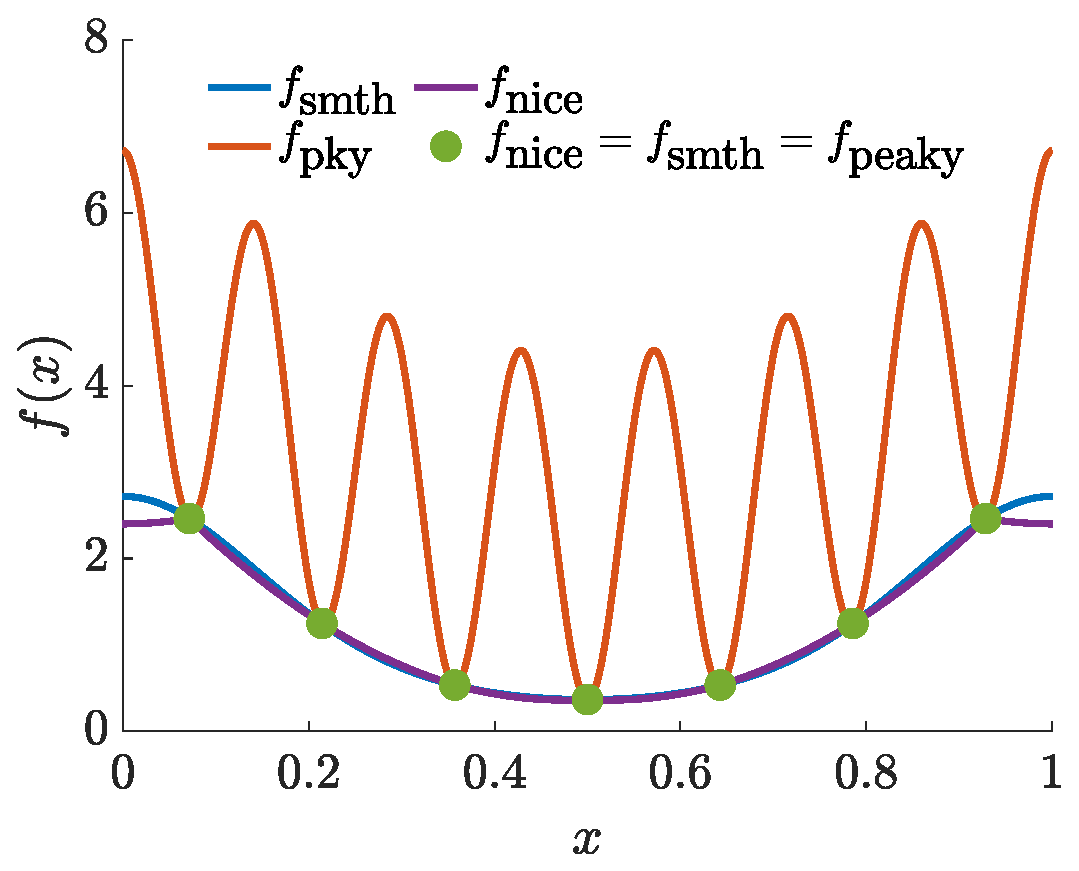
\includegraphics[width=0.8\linewidth]{figures/cone_bayes_f_real}
	%\end{subfigure}
	\caption{Example integrands 1) $f_{\NICE}$, a smooth function, 2) $f_{\PEAKY}$, a peaky function. The function values $f_{\PEAKY}(\vx_i) = f_{\NICE}(\vx_i) = f_{\TRUE}(\vx_i) $ for $i=1, \cdots, n$. This plot can be conditionally reproduced using \code{DemoCone.m}}
	\label{fig:cone_bayes_functions}
\end{figure}
\begin{figure}[ht]
	\centering
	%\begin{subfigure}[h]{0.48\linewidth}
	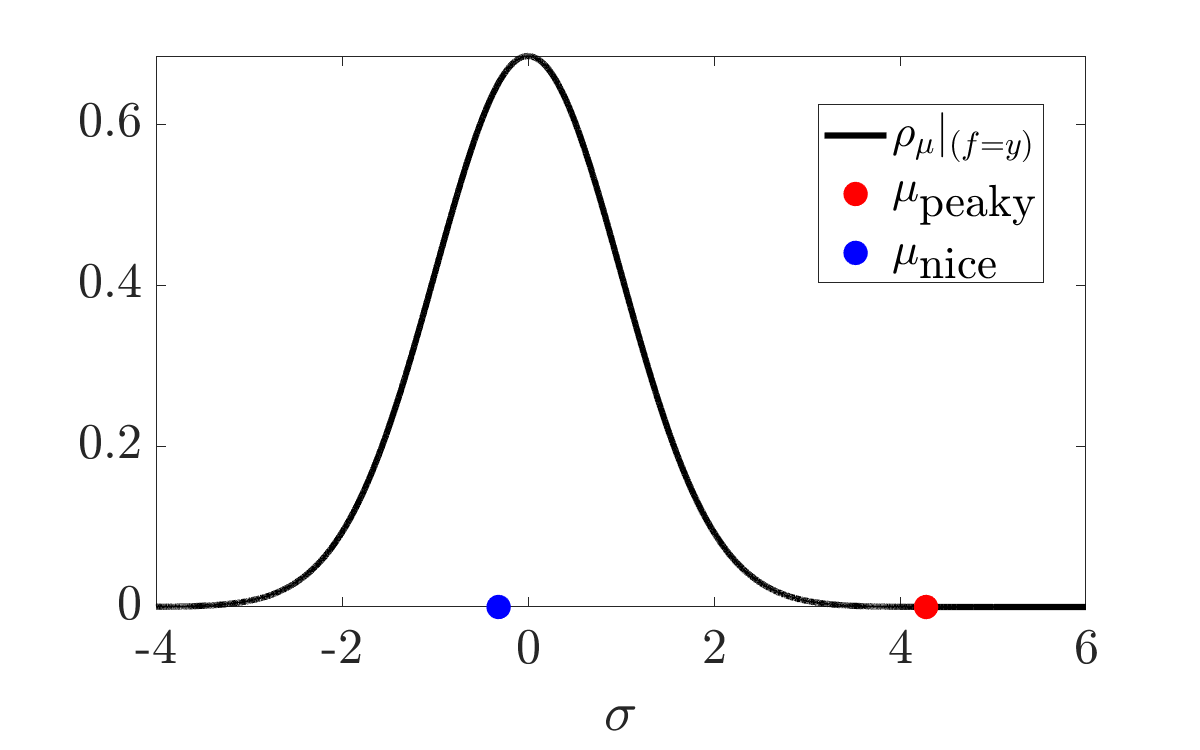
\includegraphics[width=0.8\linewidth]{figures/cone_bayes_mu_pdf}
	%\end{subfigure}
	\caption{Probability distributions showing the relative integral position of a smooth and a peaky function. $f_{\NICE}$ lies within the center 99\% of the confidence interval, and $f_{\PEAKY}$ lies on the outside of 99\% of  the confidence interval. This plot can be conditionally reproduced using \code{DemoCone.m}}
	\label{fig:cone_bayes_posterior}
\end{figure}
% Done: \JRNote{Use standard deviation $\sigma$ in x-axis.  $f_{\NICE}$ using kernel approximation} 

In \figref{fig:cone_bayes_functions}, the sampled function values
% , $\{f_{\TRUE}(\vx_i)\}_{i=1}^n$, from a smooth integrand $f_{\TRUE}$ 
are shown as dots. One can imagine these samples % $\{f(\vx_i)\}_{i=1}^n$ 
were obtained from $f_{\NICE}$, a moderately smoother function or from $f_{\PEAKY}$, a highly oscillating function. In this example, we used $a_{\PEAKY} = 2$.

When using $n=16$ rank-1 lattice points, and $r=1$ shift-invariant kernel, we get the posterior distribution of $\mu$ as shown in \figref{fig:cone_bayes_posterior}. The true integral value is shown as $\mu_{\TRUE}$ which is at the center of the plot. The integral of the peaky function $f_{\PEAKY}$ lies outside of the 99\% of the credible interval given by \eqref{eqn_prob_CI_MLE}, whereas the $\mu_{\NICE}$ falls within.

Our Bayesian cubature algorithms compute the approximate integral using only the samples of the integrand. 
Estimated integral value of our algorithm closely matches the integral of a smooth function that falls within the middle of the confidence interval. If the true integrand were to resemble the smooth approximate function then the estimated integral will be accurate.  

 

\section{Sobol' Nets and Walsh Kernels}
\label{sec:sobol_walsh}



The previous section shows an automatic Bayesian cubature algorithm using rank-1 lattice nodes and shift-invariant kernels. 
In this chapter, we demonstrate a second approach to formulate fast Bayesian transform using matching kernel and point sets. 
Scrambled Sobol' nets and Walsh kernels are paired to achieve $\Order(n^{-1 + \epsilon})$ order error convergence where $n$ is the sample size. 
Sobol' nets \cite{Sob67} are low discrepancy points, used extensively in numerical integration, simulation, and optimization. 
%Higher order digital nets with matching smoother kernels could be combined to provide higher order error convergence $\Order(N^{-\alpha + \epsilon})$ for $\alpha \ge 1$ and $\epsilon > 0$ but it is not covered in this work.
The results of this chapter can be summarized as a theorem,

% \Section{Summary}


\begin{theorem}
	Any symmetric, positive definite, digital shift-invariant covariance kernel of the form \eqref{eqn:walsh_kernel} scaled to satisfy \eqref{addAssump}, when matched with digital net data-sites, satisfies assumptions \eqref{fastcompAssump}.  The \emph{fast Walsh-Hadamard transform} (FWHT) can be used to expedite the estimates of $\vtheta$ in \eqref{thetaSimple} and the credible interval widths \eqref{fastStoppingCriterions} in $\Order(n \log n)$ operations. The cubature, $\hmu$, is just the sample mean.
\end{theorem}
We introduce the necessary concepts and prove this theorem in the remaining of this chapter.

\section{Sobol' Nets}

% Notations
% \ell - dimesnion
% i,j - point sequence index

Nets were developed to provide deterministic sample points for quasi-Monte Carlo rules \cite{Nie05a}. Nets are defined geometrically using elementary intervals, which are subintervals of the unit cube $[0,1)^d$.
The $(t,m, d)$-nets in base $b$, introduced by Niederreiter, 
%are point sets consisting of $n=b^m$ points in $[0, 1)^d$, 
whose quality is governed by $t$. Lower values of $t$ correspond to $(t,m, d)$-nets of higher quality \cite{Bald10a}.

\begin{defn}
	\label{defn:tmd_net}
	Let $\mathcal{A}$ be the set of all elementary intervals $\mathcal{A} \subset [0, 1)^d$ where
	$\mathcal{A} = \prod_{\ell=1}^d [\alpha_\ell b^{-\gamma_\ell} , (\alpha_\ell + 1) b^{-\gamma_\ell})$, 
	% with integers $d \ge 1, b \ge 2, \gamma_\ell \ge 0$,
	with $d,b,\gamma_\ell \in \naturals, b \ge 2$ 
	and $b^{\gamma_\ell}
	> \alpha_\ell \ge 0$. For $m,t \in \naturals, m \ge t \ge 0$, the point set $\mathcal{P}_m \in [0, 1)^d$ with $n = b^m$ points is a $(t, m, d)$ -- net in base $b$ if every $\mathcal{A}$ with volume $b^{t-m}$ contains $b^t$ points of $\mathcal{P}_m$.
\end{defn}

Digital $(t,m, d)$-nets are a special case of $(t,m, d)$-nets, constructed using matrix-vector multiplications over finite fields. Digital sequences are infinite length digital nets, i.e., the first $n=b^m$ points of a digital sequence comprise a digital net for all integer $m \in \naturals_0$.
% \JRNote{Higher order nets details serves no purpose}
% \begin{defn}
%A $(t,m,d)$-net in base $b$ is a set of $z_i, \; i=0,1,\dots,$ of $b^m$ points of $[0,1)^d$  with the property that every elementary interval in base $b$ of volume $b^{t-m}$ contains precisely $b^t$ points from $z_i$. Here $d \ge 1$, $b\ge 2$ and $0 \le t \le m$. 
% \end{defn}


\begin{defn}
	For any non-negative integer $i = \dots i_3 i_2 i_1(\textup{base} \, b)$, define the $\infty \times 1$ vector $\vec{\imath}$ as the vector of its digits, that is, $\vec{\imath} = (i_1, i_2, \dots)^T$. 
	For any point $z = 0.z_1 z_2 \dots (\textup{base}\, b) \in [0, 1)$, define the $\infty \times 1$ vector of the digits of $z$, that is, $\vec{z} = (z_1, z_2, \dots)^T$. 
	Let $ \mathsf{G}_1, \dots , \mathsf{G}_d$ denote predetermined $\infty \times \infty$ generator matrices. 
	The digital sequence in \textup{base} $b$ is $\{\vz_0, \vz_1, \vz_2, \dots\}$, where each $\vz_i = ( z_{i1}, \dots , z_{id})^T \in [0, 1)^d$ is defined by
	\begin{align*}
	\vec{z}_{i\ell} = \mathsf{G}_{\ell} \, \vec{\imath}, \quad \ell = 1, \dots, d, \quad i = 0, 1, \dots \;.
	\end{align*}
	The value of $t$ as mentioned in Definition \ref{defn:tmd_net} depends on the choice of $\mathsf{G}_{\ell}$.
\end{defn}



% Digital sequences are defined using digitwise operations. 
Digital nets have a group structure under digitwise addition, which is a very useful property exploited in our algorithm, especially to develop a fast Bayesian transform that speedups computations.
Digitwise addition, $\oplus$, and subtraction $\ominus$, are defined in terms of $b$-ary expansions of points in $[0, 1)^d$,
\begin{align*}
\vz \oplus \vy = \left( \sum_{j=1}^\infty [z_{\ell j} + y_{\ell j} \bmod b] b^{-j} \bmod 1 \right)_{\ell=1}^d,
\\
\vz \ominus \vy = \left( \sum_{j=1}^\infty [z_{\ell j} - y_{\ell j} \bmod b] b^{-j} \bmod 1 \right)_{\ell=1}^d,
\end{align*}
where
\begin{align*}
\vz = \left( \sum_{j=1}^{\infty} z_{\ell j}b^{-j}\right)_{\ell=1}^d, \quad
\vy = \left( \sum_{j=1}^{\infty} y_{\ell j}b^{-j}\right)_{\ell=1}^d, \quad
z_{\ell j}, y_{\ell j} \in \{0,\cdots,b-1\}.
\end{align*}



Similarly for integer values in $\naturals_0^d$, the digitwise addition, $\oplus$, and subtraction $\ominus$, are defined in terms of their $b$-ary expansions,
\begin{align*}
\vk \oplus \vl = \left( \sum_{j=0}^\infty [k_{\ell j} + l_{\ell j} \bmod b] b^{j} \bmod 1 \right)_{\ell=1}^d,
\\
\vk \ominus \vl = \left( \sum_{j=0}^\infty [k_{\ell j} - l_{\ell j} \bmod b] b^{j} \bmod 1 \right)_{\ell=1}^d,
\end{align*}
where
\begin{align*}
\vk = \left( \sum_{j=0}^{\infty} k_{\ell j}b^{j}\right)_{\ell=1}^d, \quad
\vl = \left( \sum_{j=0}^{\infty} l_{\ell j}b^{j}\right)_{\ell=1}^d, \quad
\vk_{\ell j}, \vl_{\ell j} \in \{0,\cdots,b-1\}.
\end{align*}

Let $\{\vz_i\}_{i=0}^{b^m-1}$ be a digital net. Then
\begin{align*}
\forall i_1, i_2 \in \{0,\cdots,b^m-1\}, \quad \vz_{j_1} \oplus \vz_{i_2} = \vz_{i_3}, \quad \text{for some} \; i_3 \in \{0,\cdots,b^m-1\}.
\end{align*}

The following very useful result, which will be further used to obtain the fast Bayesian transform, arises from the fundamental property of digital nets.

\begin{lemma}
	\label{lemma:digital_net_prop}
	Let $\{\vz_i\}_{i=0}^{b^{m}-1}$ be the digital-net and the corresponding digitally shifted net be $\{\vx_i\}_{i=0}^{b^{m}-1}$, i.e.,
	\begin{align*}
	\vec{x}_{i \ell} = \vec{z}_{i \ell} + \vec{\Delta}_l \bmod 1,
	\end{align*}
	where $\vec{x}_{i \ell}$ is the $\ell$th component of $i$th digital net and $\vec{\Delta}_{\ell}$ is the digital shift for the $\ell$th component. 
	% Let $\vx_i, \vx_j$ be digitally shifted digital nets and $\vz_i, \vz_j$ be the corresponding un-shifted digital nets, 
	Then,
	\begin{align}
	\label{eqn:digital_shift_prop}
	\vx_i \ominus \vx_j = \vz_i \ominus \vz_j = \vz_{i \ominus j}, \quad \forall i,j \in \naturals_0. 
	\end{align}
	Also the digital subtraction is symmetric,
	\begin{align}
	\label{eqn:digital_net_symmetric_prop}
	\vx_i \ominus \vx_i = \boldsymbol{ 0}, \qquad 
	\vx_i \ominus \vx_j = \vx_j \ominus \vx_i, \quad \forall i,j \in \naturals_0.
	\end{align}
\end{lemma}

\begin{proof}
	
	The proof can be obtained from the definition of digital nets which stated that the digital nets are obtained using generator matrices, $\vec{z}_{i \ell} = \mG_{\ell} \, \vec{\imath} \bmod b$. Rewriting the subtraction using the generating matrix provides the result,
	\begin{align*}
	\vec{z}_{i \ell} - \vec{z}_{j\ell} \bmod b & = (\mG_{\ell} \vec{\imath} \bmod b) - (\mG_{\ell} \vec{\jmath} \bmod b) \\
	& = (\mG_{\ell} \vec{\imath} - \mG_{\ell} \vec{\jmath} ) \bmod b \\
	& = \mG_{\ell} (\vec{\imath} - \vec{\jmath} ) \bmod b \\
	& = \mG_{\ell} (\overrightarrow{i \ominus j} ) \bmod b \\
	& = \vec{z}_{i \ominus j \; {\ell}}.
	\end{align*}
	The rest of the lemma is obvious from the definition of digital nets.
\end{proof}

% \JRNote{Define and explain scrambling}
We chose digitally shifted and scrambled nets \cite{HicYue00} for our Bayesian cubature algorithm. Digital shifts help to avoid having nodes at the origin, similar to the random shift used with lattice nodes.
\iffalse
Let $\{\vx_0, \vx_1, \vx_2, ...\}$ denote the randomly scrambled version of the original sequence $\{\vz_0, \vz_1, \vz_2, \dots \}$. Let $x_{i{\ell}j}$ denote the $j$\textup{th} digit of the $\ell$\textup{th} component of $\vx_i$, and similarly for $z_{i{\ell}j}$. Then
\begin{align*}
x_{i{\ell}1} = \pi_{\ell}( z_{i{\ell}1}), \quad x_{i{\ell}2} = \pi_{z_{i{\ell}1}} ( z_{i{\ell}2}), \quad x_{i{\ell}3} = \pi_{z_{i{\ell}1}, z_{i{\ell}2}} ( z_{i{\ell}3}), \quad \dots , \\
x_{i{\ell}j} = \pi_{z_{i{\ell} 1}, z_{i{\ell}2}, \dots, z_{i{\ell}j-1}} ( z_{i{\ell}j}), \quad \dots , \qquad \qquad \qquad
\end{align*}
where the $\pi_{a_1a_2 \dots}$ are random permutations of the elements in $\{0,\dots,b-1\}$ chosen uniformly and mutually independent. 
\fi
Scrambling helps to eliminate bias while retaining the low-discrepancy properties.
A proof that a scrambled net preserves the property of $(t, m, d)$-net almost surely can be found in Owen \cite{Owe95}. The scrambling method proposed by Matou\v{s}ek \cite{Mat98} is preferred since it is more efficient than the Owen's scrambling.

Sobol' nets \cite{Sob76} are a special case of $(t,m, d)$-nets when base $b=2$. 
An example of $64$ Sobol' nets in $d=2$ is given in \figref{fig:sobol-fig}.  The even coverage of the unit cube is ensured by a well chosen generating matrix.  The choice of generating vector is typically done offline by computer search.  See \cite{KuoNuyens2016} and \cite{NuySoft} for more on generating matrices. We use randomly scrambled and digitally shifted Sobol' sequences in this research \cite{HonHic00a}. 

\begin{figure}[htp]
	\label{fig:sobol-fig}
	\centering
	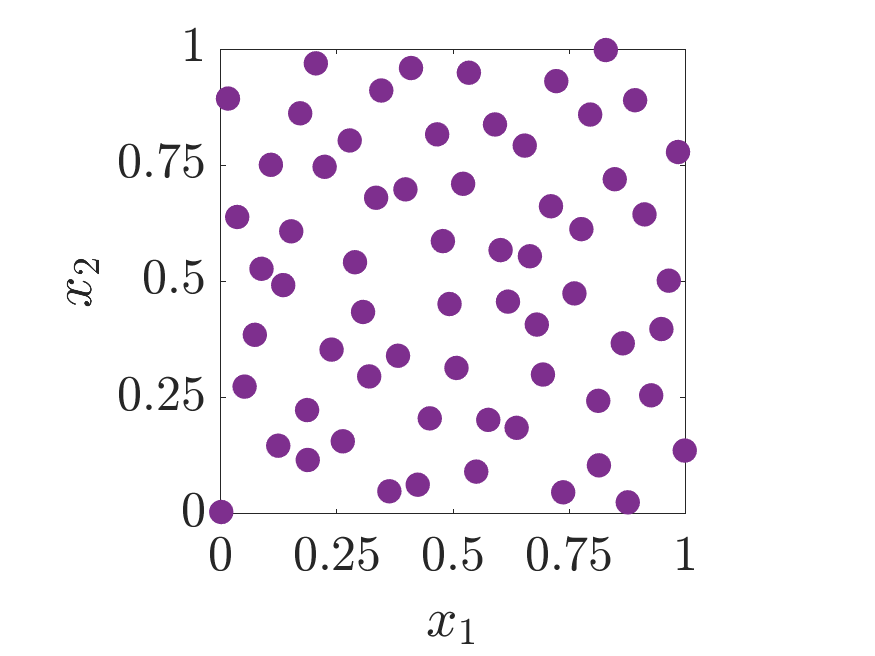
\includegraphics[width=0.8\linewidth]{figures/SSobolPoints}
	\caption{Example of a scrambled Sobol' node set  in $d=2$.  This plot can be reproduced using \code{PlotPoints.m}. \label{sobolfig} }
\end{figure}


\section{Walsh Kernels}

Walsh kernels are product kernels based on the Walsh functions. We introduce the necessary concepts in this section.

\subsection{Walsh functions}
Like the Fourier transform used with lattice points (Section~\ref{sec:shift_invar_kern}), the Walsh-Hadamard transform, which we will simply call Walsh transform, is used for the digital nets. The Walsh transform is defined using Walsh functions. Recall $\naturals_0 := \lbrace 0,1,2,\cdots \rbrace$.
The one-dimensional Walsh functions in base $b$ are defined as
\begin{align}
\label{eqn:walsh_func}
\textup{wal}_{b,k}(x) := e^{2\pi \sqrt{-1} (x_1 k_0 + x_2 k_1 + \cdots)/b} 
=
e^{2\pi \sqrt{-1} {\vec{k}}^T{\vec{x}}/b},
\end{align}
for $x \in [0,1)$ and $k \in \naturals_0$ and the unique base $b$ expansions 
$x = \sum_{j \ge 1} x_j b^{-i} = (0.x_1 x_2 \cdots)_b$, $\vec{x} =  (x_1,x_2,\cdots )^T$
$k = \sum_{j \ge 0} k_j b^{j} = ( \cdots k_1 k_0)_b$, $\vec{k} =  (k_0,k_1,\cdots )^T$, and ${\vec{k}}^T{\vec{x}} = x_1 k_0 + x_2 k_1 + \cdots$
where the number of digits used in \eqref{eqn:walsh_func} are limited to the length required to represent $x$ or $k$, i.e., $\max \left( {\ceil{ -\log_b{x}}, \ceil{\log_b{k}}  } \right)$.
% with $n$ at least as large as the number of digits to represent $x$ or $k$.
Multivariate Walsh functions are defined as the product of the one-dimensional Walsh functions,
\begin{align*}
\textup{wal}_{b,\vk} (\vx) := \prod_{\ell=1}^d \textup{wal}_{b,k_\ell} (x_\ell
)
\end{align*}
As shown in \eqref{eqn:walsh_func}, for the case of $b=2$, the Walsh functions only take the values in $\{1, -1\}$, i.e., $\textup{wal}_{b,\vk} : [0,1)^d \to {\{-1, 1\}} , \; k \in \naturals_0^d$. Walsh functions form an orthonormal basis of the Hilbert space $L^2[0,1)^d$,
\begin{align*}
\int_{[0,1)^d}
\textup{wal}_{b,\vl} (\vx) \textup{wal}_{b,\vk}(\vx) \dx = \delta_{\vl, \vk}, \quad \forall \vl, \vk \in \naturals_0^d
\end{align*}
Digital nets are designed to integrate certain Walsh functions without error.
Thus our Bayesian cubature algorithm integrates linear combinations of % these ideal integrands
certain Walsh functions without error. Functions that are well approximated by such linear combinations are then integrated with small errors.

% \JRNote{separate paragraph}
In this research we use Sobol' nodes which are digital nets with base $b=2$. So here afterwards base $b=2$ is assumed. % if not specified or the notation is dropped.  
In this case, the Walsh function is simply $$\textup{wal}_{2,\vk} (\vx) = (-1)^{\vec{\vk}^T \vec{\vx}}.$$

\subsection{Walsh kernels}
Consider the covariance kernels of the form,
\begin{align}
\label{eqn:digital_shift_in_kernel}
C_{\vtheta}(\vx, \vt) = K_{\vtheta} (\vx \ominus \vt) 
\end{align}
where $\ominus$ is bitwise subtraction.
This is called a \emph{digitally shift invariant kernel} because shifting both arguments of the covariance function by the same amount leaves the value unchanged. By a proper scaling of the function $K_{\vtheta}$, it follows that assumption \eqref{addAssump} is satisfied. The function $K_{\vtheta}$ must be of the form that ensures that $C_{\vtheta}$ is symmetric and positive definite, as assumed in \eqref{FJH:eq:CondPosDef}. We drop the ${\vtheta}$ sometimes to make the notation simpler.
The Walsh kernels are of the form,
\begin{align}
\label{eqn:walsh_kernel}
K_{\vtheta} (\vx \ominus \vt) =  
\prod_{\ell=1}^d  1 + \eta_\ell \omega_{r} (x_\ell \ominus t_\ell), \quad \veta = (\eta_1, \cdots, \eta_d), \quad \vtheta = (r, \veta)
\end{align}
where $r$ is the kernel order, $\veta$ is the kernel shape parameter, and
\begin{align*}
\omega_r(x) = \sum_{k=1}^\infty 
\frac{\textup{wal}_{2,k}(x) }{2^{2r \lfloor \log_2 k \rfloor}}.
\end{align*}
Explicit expression is available for $\omega_{r}$ in the case of order $r=1$ \cite{Nuyens2013}, % and Hilbert space setup,
\begin{align}
\label{eqn:omega1}
\omega_1(x) 
% &= \prod_{l=1}^d \sum_{k=1}^\infty 
% \frac{\textup{wal}_{b,k}(x_l) }{b^{2 \lfloor \log_b k \rfloor}} 
= 6\left( \frac 16 - 2^{\lfloor \log_2 x \rfloor -1 }\right).
\end{align}



\begin{figure}
	\centering
	\includegraphics[width=0.9\linewidth]{"figures/walsh_kernel dim_1"}
	\caption[Walsh kernel]{Walsh kernel of order $r=1$ in dimension $d=1$. This figure can be reproduced using \code{plot\_walsh\_kernel.m}. %\JRNote{remove $r=1$ in the figure}
	}
	\label{fig:walshkernel-dim1}
\end{figure}

The \figref{fig:walshkernel-dim1} shows the Walsh kernel \eqref{eqn:walsh_kernel} of order $r=1$ in the interval $[0,1)$. Unlike the shift-invariant kernels used with lattice nodes, low order Walsh kernels are discontinuous and are only piecewise constant. Smaller $\eta_\ell$ implies lesser variation in the amplitude of the kernel. Also, the Walsh kernels are digitally shift invariant but not periodic.

\section{Eigenvectors}

We show the eigenvectors $\mV$ in \eqref{eqn:ftk_factor} of the Gram matrix formed by the covariance kernel \eqref{eqn:walsh_kernel} and Sobol' nets are the columns of the Walsh-Hadamard matrix. First we introduce the necessary concepts.

\subsection{Walsh transform}
% \JRNote{add subsection for walsh transform, define and explain.}
The Walsh-Hadamard transform (WHT) is a generalized class of discrete Fourier transform (DFT) and is much simpler to compute than the DFT. The WHT matrices are comprised of only $\pm 1$ values, so the computation usually involves only ordinary additions and subtractions. Hence, the WHT is also sometimes called the integer transform. In comparison, the DFT that was used with lattice nodes,  uses complex exponential functions and the computation involves complex, non-integer multiplications. 

The WHT involves multiplications by $2^m \times 2^m$ Walsh-Hadamard matrices, which is constructed recursively, starting with $\mH^{(0)} = 1$,
\begin{align}
\nonumber
\arraycolsep=1.4pt\def\arraystretch{0.9}
\mH^{(1)} &=
\begin{pmatrix}
1 & 1 \\ 1 & -1
\end{pmatrix}, \\
\nonumber
\mH^{(2)} &= 
\begin{pmatrix}
1 & 1 & 1 & 1 \\ 
1 & -1 & 1 & -1 \\
1 & 1 & -1 & -1 \\ 
1 & -1 & -1 & 1 \\
\end{pmatrix}, \\
\nonumber
& \qquad \vdots
\\
\label{eqn:hadamard_matrix}
\mH^{(m)} &= 
\begin{pmatrix}
\mH^{(m-1)} & \mH^{(m-1)} \\ \mH^{(m-1)} & -\mH^{(m-1)}
\end{pmatrix} 
= \underbrace{\mH^{(1)} \bigotimes \cdots \bigotimes \mH^{(1)}}_{m \ \text{times}} 
= \mH^{(1)} \bigotimes \mH^{(m-1)}
\end{align}
where $\bigotimes$ is Kronecker product. Alternatively for base $b=2$, these matrices can be  directly obtained by,
\begin{align*}
\mH^{(m)} % = \bigg(\exp(\pi \sqrt{-1} \vec{\imath}_m^T\vec {\jmath}_m) \bigg)_{i,j=0}^{n-1}  
= \bigg((-1)^{(\vec{\imath}^T \vec{\jmath})} \bigg)_{i,j=0}^{2^m-1},
\end{align*}
where the notation $\vec{\imath}^T \vec{\jmath}$ indicates the bitwise dot product. 

\iffalse
An example of Walsh matrix of length $n=8$ is given in Table~\ref{tab:hadamard_matrix}. 
\begin{table} % 
	% \centering
	\arraycolsep=1pt\def\arraystretch{0.8}
	\[
	%\arraycolsep=1.4pt\def\arraystretch{0.9}
	\begin{array}{c|@{\quad}r@{\quad}r@{\quad}r@{\quad}r@{\quad}r@{\quad}r@{\quad}r@{\quad}r@{\quad}r}
	\hhline{=========}
	%\vspace{-1.5ex}
	\text{Zero crossings} & \multicolumn{8}{l}{\text{Walsh function values}} \\
	\hline
	0&	1&  1&  1&  1&  1&  1&  1&  1 \\
	4&	1& -1& -1&  1&  1& -1& -1&  1 \\
	6&	1& -1&  1& -1& -1&  1& -1&  1 \\
	2&	1&  1& -1& -1& -1& -1&  1&  1 \\
	3&	1&  1& -1& -1&  1&  1& -1& -1 \\
	7&	1& -1&  1& -1&  1& -1&  1& -1 \\
	5&	1& -1& -1&  1& -1&  1&  1& -1 \\
	1&	1&  1&  1&  1& -1& -1& -1& -1
	\end{array}
	\]
	\vspace{-5ex}
	\caption{Walsh transform matrix of for $n=8$, in Hadamard order  \label{tab:hadamard_matrix}}	   
\end{table}
\fi


\subsection{Eigenvectors of $\mC$ are columns of Walsh-Hadamard matrix}
\label{sec:eigenvector_hadamard}
The Gram matrix $\mCtheta$ formed by Walsh kernels and Sobol' nodes have a special structure called  block-Toeplitz, which can be used to construct the fast Bayesian transform. 
A Toeplitz matrix is a diagonal-constant matrix in which each descending diagonal from left to right is constant. A block Toeplitz matrix is a special block matrix, which contains blocks that are repeated down the diagonals of the matrix.
%, as a Toeplitz matrix has elements repeated down the diagonal. 
We prove that the eigenvectors of $\mCtheta$ are columns of a Walsh-Hadamard matrix in two theorems. 

\begin{theorem}
	\label{thrm:block-toeplitz}
	Let $\left(\vx_i\right)_{i=0}^{n-1}$ be digitally shifted Sobol' nodes and $K$ be any function,
	% positive definite kernel function such as \eqref{eqn:omega1} which matches Sobol' nodes.
	then the Gram matrix,
	\begin{align*}
	\mCtheta = \bigl(C(\vx_i, \vx_j)\bigr)_{i,j=0}^{n-1} &= \bigl(K(\vx_i \ominus \vx_j)\bigr)_{i,j=0}^{n-1},   \\ & \text{where} \quad \quad n=2^m, \quad C(\vx, \vt) = K(\vx \ominus \vt), \quad  \vx, \vt \in [0,1)^d, \qquad
	\end{align*}
	is a $2\times 2$ block-Toeplitz matrix and all the sub-blocks and their sub-sub-blocks, etc. are also $2\times 2$ block-Toeplitz. 
\end{theorem}

%\Subsubsection
\begin{proof}
	
	
	%\textbf{Proof of Theorem \ref{thrm:block-toeplitz}}: 
	We prove this theorem by induction. Let $\mC_{\vtheta}^{(m)}$ denote the Gram matrix of size $2^m \times 2^m$.
	The relation between sub-block matrices can be deciphered using the properties of digital nets.
	To help with the proof of block-Toeplitz structure, consider the digital net properties \eqref{eqn:digital_shift_prop},  \eqref{eqn:digital_net_symmetric_prop},
	%\begin{align*}
	%\bigl(K(\vz_i \ominus \vz_j)\bigr)_{i,j=0}^{n-1}.
	%\end{align*}
	% Now we can prove the block-Toeplitz structure using these properties and facts \JRNote{add refs to properties}.
	and notations,
	\begin{align*}
	\mK^{(m)} &:= 
	\begin{pmatrix}
	K({\vz_{i} \ominus \vz_{j}})
	\end{pmatrix}_{i,j=0}^{2^{m}-1}
	=
	\begin{pmatrix}
	K({\vz_{i \ominus j}})
	\end{pmatrix}_{i,j=0}^{2^{m}-1}, \quad m=1,2,\cdots,
	\\
	\mK^{(m,q)} &:= 
	\begin{pmatrix}
	K({\vz_{i \ominus j + q 2^m}})
	\end{pmatrix}_{i,j=0}^{2^{m}-1},
	\quad 
	q = 0,1,\cdots .
	\end{align*} 
	These two notations are related by $\mK^{(m)} = \mK^{(m,0)}$. 
	Please note that $\mC_{\vtheta}^{(m)} = \mK^{(m,0)}$.
	% Since the digitally shift invariant kernel are used in this research. %, it is sufficient to prove $\mK^{(m,q)}$ as a $2\times 2$ block-Toeplitz. 
	We will prove $\mK^{(m,q)}$ is a $2\times 2$ block-toeplitz matrix for all $m \in \naturals, q \in \naturals$.
	
	% This notation is convenient for the proof as shown below.
	
	\iffalse
	As the first step, we verify the property holds for $m=0$,
	\begin{align*}
	\mK^{(0,q)} &= \begin{pmatrix}
	K(\vz_{0 \ominus 0 + q 2^0})  
	\end{pmatrix} = 
	\begin{pmatrix}
	K(\vz_{q})
	\end{pmatrix}, \quad \text{by \eqref{eqn:digital_shift_prop}},
	\end{align*} thus by definition $\mK^{(0,q)}$ is a block-Toeplitz.
	\fi 
	
	\iftrue
	As the first step, we verify the property holds for $m=1$,
	\begin{align*}
	\mK^{(1, q)} &= \begin{pmatrix}
	K(\vz_{0 \ominus 0 + q 2^1}) & K(\vz_{1 \ominus 0 + q 2^1})  \\
	K(\vz_{0 \ominus 1 + q 2^1}) & K(\vz_{1 \ominus 1 + q 2^1})  
	\end{pmatrix} = 
	\begin{pmatrix}
	K(\vz_{2q}) & K(\vz_{1 + 2q}) \\ K(\vz_{1 + 2q}) & K(\vz_{2q})
	\end{pmatrix}, \quad \text{by \eqref{eqn:digital_shift_prop}}
	\end{align*} has diagonal elements repeated. Thus by definition, it is a $2\times 2$ block-Toeplitz.
	\fi 
	
	\iffalse
	Similarly, the property can be verified for $\mC^{(2)}$, 
	\begin{align*}
	\mC^{(2)} &= 
	\begin{pmatrix}
	K_{z_{(i \ominus j )}}
	\end{pmatrix}_{i,j=0}^{2^2-1}
	=
	\begin{pmatrix}
	K(\vz_{0 \ominus 0}) & K(\vz_{1 \ominus 0}) & K(\vz_{2 \ominus 0}) & K(\vz_{3 \ominus 0}) \\
	K(\vz_{0 \ominus 1}) & K(\vz_{1 \ominus 1}) & K(\vz_{2 \ominus 1}) & K(\vz_{3 \ominus 1}) \\
	K(\vz_{0 \ominus 2}) & K(\vz_{1 \ominus 2}) & K(\vz_{2 \ominus 2}) & K(\vz_{3 \ominus 2}) \\
	K(\vz_{0 \ominus 3}) & K(\vz_{1 \ominus 3}) & K(\vz_{2 \ominus 3}) & K(\vz_{3 \ominus 3}) 
	\end{pmatrix} \\
	& = 
	\begin{pmatrix}
	\begin{pmatrix}
	K(\vz_{0}) & K(\vz_{1}) \\
	K(\vz_{1}) & K(\vz_{0})
	\end{pmatrix} &
	\begin{pmatrix}
	K(\vz_{2}) & K(\vz_{3}) \\
	K(\vz_{3}) & K(\vz_{2}) 
	\end{pmatrix} \\
	\begin{pmatrix}
	K(\vz_{2}) & K(\vz_{3}) \\
	K(\vz_{3}) & K(\vz_{2}) 
	\end{pmatrix} &
	\begin{pmatrix}
	K(\vz_{0}) & K(\vz_{1}) \\
	K(\vz_{1}) & K(\vz_{0})
	\end{pmatrix} 
	\end{pmatrix}, \quad \text{by \eqref{eqn:digital_shift_prop}, \eqref{eqn:digital_net_symmetric_prop}}
	\\
	& =
	\begin{pmatrix}
	\mC^{(1)} & \mC^{(1,1)} \\
	\mC^{(1,1)} & \mC^{(1)}
	\end{pmatrix},
	\end{align*}
	is a block-Toeplitz as it is obvious from the block structure depicted. 
	\fi
	% Here we used the notation $\mC^{(1,1)}$ to indicate the additional operation involved in the matrix.
	% Where the matrix $\mC^{(1,1)}$ is obtained using the following shift operation.
	
	Now assume that $\mK^{(m,q)}$ is block-Toeplitz.
	% Please note if $\mK^{(m,0)}$ is block-Toeplitz then $\mK^{(m,q)}$ is also a block-Toeplitz for all $q \in \naturals_0$. 
	% This is due to the fact that $i \oplus 2^m \ominus j = i \ominus j \ominus 2^m = i \ominus j \oplus 2^m $ for $i,j=0,\cdots,2^{m-1}$ since $i \ominus j < 2^{m-1}$.
	% Assuming $\mK^{(m, q)}$ is a block-Toeplitz, 
	We need to prove $\mK^{(m+1, q)}$ is also a $2\times 2$ block-Toeplitz. Let $n=2^m$,
	\begin{align*}
	\mK^{(m+1)} &= 
	\begin{pmatrix}
	K(\vz_{0    \ominus 0}) & \hdots & K(\vz_{0    \ominus n-1}) & K(\vz_{0    \ominus n}) & \hdots & K(\vz_{0    \ominus 2n-1}) \\
	\vdots             & \vdots &             \vdots          &           \vdots      & \vdots &             \vdots         \\
	K(\vz_{n-1  \ominus 0}) & \hdots & K(\vz_{n-1  \ominus n-1}) & K(\vz_{n-1  \ominus n}) & \hdots & K(\vz_{n-1  \ominus 2n-1}) \\
	K(\vz_{n    \ominus 0}) & \hdots & K(\vz_{n    \ominus n-1}) & K(\vz_{n    \ominus n}) & \hdots & K(\vz_{n    \ominus 2n-1}) \\
	\vdots      & \vdots &             \vdots        &             \vdots      & \vdots &             \vdots         \\
	K(\vz_{2n-1 \ominus 0}) & \hdots & K(\vz_{2n-1 \ominus n-1}) & K(\vz_{2n-1 \ominus n}) & \hdots & K(\vz_{2n-1 \ominus 2n-1}) 
	\end{pmatrix} 
	\\
	& = 
	\begin{pmatrix}
	\begin{pmatrix}
	K(\vz_{  0   }) & \hdots & K(\vz_{ n-1}) \\
	\vdots          & \vdots &    \vdots     \\
	K(\vz_{ n-1  }) & \hdots & K(\vz_{ 0 })
	\end{pmatrix}
	& 
	\begin{pmatrix}
	K(\vz_{ n})     & \hdots & K(\vz_{ 2n-1}) \\
	\vdots          & \vdots &     \vdots     \\
	K(\vz_{ 2n-1 }) & \hdots & K(\vz_{ n })   
	\end{pmatrix}
	\\
	\begin{pmatrix}
	K(\vz_{ n})     & \hdots & K(\vz_{ 2n-1}) \\
	\vdots          & \vdots &     \vdots     \\
	K(\vz_{ 2n-1 }) & \hdots & K(\vz_{ n })   
	\end{pmatrix}
	&
	\begin{pmatrix}
	K(\vz_{  0   }) & \hdots & K(\vz_{ n-1}) \\
	\vdots          & \vdots &    \vdots     \\
	K(\vz_{ n-1  }) & \hdots & K(\vz_{ 0 })
	\end{pmatrix}
	\end{pmatrix} 
	\\
	& =
	\begin{pmatrix}
	\mK^{(m)} & \mK^{(m,1)} \\ \mK^{(m,1)} & \mK^{(m)}
	\end{pmatrix}
	\end{align*}
	is a $2\times 2$ block-Toeplitz, where we used the properties  \eqref{eqn:digital_shift_prop}, \eqref{eqn:digital_net_symmetric_prop} and facts $2n-1 \ominus n = n-1$, $2n-1 \ominus n-1 = n$, and $n \ominus n-1 = 2n-1$. 
	Thus $\mK^{(m+1)}$ is a $2\times2$ block-Toeplitz. 
	Similarly 
	\begin{align*}
	\mK^{(m+1,q)} 
	& =
	\begin{pmatrix}
	\mK^{(m,q)} & \mK^{(m,q+1)} \\ \mK^{(m,q+1)} & \mK^{(m,q)}
	\end{pmatrix}
	\end{align*}
	is a $2\times2$ block-Toeplitz. 
	%\end{itemize}
	Thus $\mC_{\vtheta}^{(m)}$ of size $2^m\times 2^m$, for $m \in \naturals$, is a $2\times2$ block-Toeplitz and every block and it's sub-blocks of size $2^p, \; p \in \naturals, \; p \le m$ are also $2\times2$ block-Toeplitz.
\end{proof}

%%%%%%%%%%%%%%%%%%%%%%%%%%%%%%%%%%%%%%%%%%%%%%%%%%%%%%%%%%%%%%%%%%%%%%%%%%%%%%%

\iffalse
Some additional properties
$\bigl( K(z_{i \ominus j})\bigr)_{i=2^{l+1}q, \; j=2^{l+1}s}^{2^{l+1}{(q+1)}, \; 2^{l+1}{(s+1)}} $
\fi



\iffalse
Now we prove every arbitrary sub-block is also block-Toeplitz: 
\begin{itemize}
	\item For $l=1$
	\begin{align*}
	\bigl( K(z_{i \ominus j})\bigr)_{i=2q, \; j=2s}^{2q+1, 2s+1}, \quad q,s=0,1,\cdots,
	\end{align*}
	is a block-Toeplitz since
	\begin{align*}
	\begin{pmatrix}
	K(z_{2q \ominus 2s}) & K(z_{2q \ominus (2s +1)}) \\
	K(z_{(2q+1) \ominus 2s}) & K(z_{(2q+1) \ominus (2s +1)}) 
	\end{pmatrix}
	=
	\begin{pmatrix}
	K(z_{2q \ominus 2s}) & K(z_{1 + (2q \ominus 2s)}) \\
	K(z_{1 + (2q \ominus 2s)}) & K(z_{ 2q \ominus 2s}) 
	\end{pmatrix}
	\end{align*}
	where we used the facts $(2q+1) \ominus (2s+1) = 2q \ominus 2s$ and $(2q+1) \ominus 2s = 1 + 2q \ominus 2s$.
	
	\item \ldots
	
	\item Assuming for $2^{l}$ is a block-Toeplitz then need to prove for $2^{l+1}$ 
	\begin{align*}
	\bigl( K(z_{i \ominus j})\bigr)_{i=2^{l+1}q, \; j=2^{l+1}s}^{2^{l+1}(q+1)-1, \; 2^{l+1}(s+1)-1}, \quad q,s=0,1,\dots,
	\end{align*}
	is a block-Toeplitz.
	
	\begin{align*}
	\mC &=
	\begin{pmatrix}
	\bigl( K(z_{i \ominus j})\bigr)_{i=\ia, \; j=\ja }^{\ib, \; \jb} & \bigl( K(z_{i \ominus j})\bigr)_{i=\ia, \; j=\jc }^{\ib, \; \jd} \\
	\bigl( K(z_{i \ominus j})\bigr)_{i=\ic, \; j=\ja }^{\id, \; \jb} & \bigl( K(z_{i \ominus j})\bigr)_{i=\ic, \; j=\jc }^{\id, \; \jd}
	\end{pmatrix} \\
	& =
	\begin{pmatrix}
	\bigl( K(z_{i \ominus j})\bigr)_{i=\ia, \; j=\ja }^{\ib, \; \jb} & \bigl( K(z_{i \ominus j})\bigr)_{i=\ia, \; j=\jc }^{\ib, \; \jd} \\
	\bigl( K(z_{i \ominus j})\bigr)_{i=\ia, \; j=\jc }^{\ib, \; \jd} & \bigl( K(z_{i \ominus j})\bigr)_{i=\ia, \; j=\ja }^{\ib, \; \jb}
	\end{pmatrix}
	\end{align*}
	is a block-Toeplitz. Where we used the facts
	\begin{align*}
	% \ic \ominus \jc 
	& 2^{l}(2q+1) \ominus 2^{l}(2s+1) = 2^{l}(2q) \ominus 2^{l}(2s) = 2^{l+1}(q) \ominus 2^{l+1}(s) \\
	% \jd \ominus \ic
	&2^{l+1}(s+1)-1 \, \ominus 2^{l}(2q + 1) % = 2^{l}(2s+1 + 1)-1 \ominus 2^{l}(2q + 1) 
	= 2^{l}(2s+1)-1 \ominus 2^{l+1}q.
	\end{align*}
	
	Thus $\mCtheta^{(m)}$ is a block-Toeplitz and every block its and sub-blocks are also block-Toeplitz.
	
	
\end{itemize}
\fi


\begin{theorem}
	\label{thrm:hadamard_eigenvector}
	The Walsh-Hadamard matrix $\mH^{(m)}$ factorizes $\mC_{\vtheta}^{(m)}$, so that the columns of Walsh-Hadamard matrix are the eigenvectors of $\mC_{\vtheta}^{(m)}$, i.e.,
	\begin{align*}
	\mH^{(m)} \mC_{\vtheta}^{(m)}  = \mLambda^{(m)} \mH^{(m)}, \quad m \in \naturals. 
	\end{align*}
\end{theorem}

\begin{proof}
	
	Again, we use the proof-by-induction technique to show that the Walsh-Hadamard matrix factorizes $\mK^{(m,q)}$.
	\iffalse
	We can easily see the Hadamard matrix $\mH^{(0)}$ diagonalizes $\mC^{(0)}$,
	\begin{align*}
	\mH^{(0)} \mC^{(0)} &= 
	\begin{pmatrix}
	1 
	\end{pmatrix}
	\begin{pmatrix}
	K(\vz_{0}) 
	\end{pmatrix}
	\\
	% & = \begin{pmatrix} K(\vz_{0})+K(\vz_{1}) & K(\vz_{0})+K(\vz_{1}) \\ K(\vz_{0})-K(\vz_{1}) & K(\vz_{1})-K(\vz_{0}) \end{pmatrix} \\ 
	& = 
	\begin{pmatrix}
	K(\vz_{0})
	\end{pmatrix}
	\begin{pmatrix}
	1 
	\end{pmatrix}
	\\ 
	% & = \begin{pmatrix} K(\vz_{0})+K(\vz_{1}) & 0 \\ 0 & K(\vz_{0})-K(\vz_{1}) \end{pmatrix} \mH^{(1)} \\
	&= \mLambda^{(0)} \mH^{(0)},
	\end{align*}
	where $\mLambda^{(0)}$ is a diagonal matrix, thus $\mH^{(0)}$ diagonalizes $\mC^{(0)}$.
	\fi
	We can easily see the Hadamard matrix $\mH^{(1)}$ diagonalizes $\mK^{(1,q)}$,
	\begin{align*}
	\mH^{(1)} \mK^{(1,q)} &= 
	\begin{pmatrix}
	1 &  1 \\ 1 & -1
	\end{pmatrix}
	\begin{pmatrix}
	K(\vz_{0 + q2^1}) & K(\vz_{1 + q2^1}) \\ K(\vz_{1 + q2^1}) & K(\vz_{0 + q2^1})
	\end{pmatrix}, \quad \text{by Theorem \ref{thrm:block-toeplitz}} 
	\\
	& = \begin{pmatrix} K(\vz_{2q})+K(\vz_{2q+1}) & K(\vz_{2q})+K(\vz_{2q+1}) \\ K(\vz_{2q})-K(\vz_{2q+1}) & K(\vz_{2q+1})-K(\vz_{2q}) \end{pmatrix} \\ 
	& = \begin{pmatrix} K(\vz_{2q})+K(\vz_{2q+1}) & 0 \\ 0 & K(\vz_{2q})-K(\vz_{2q+1}) \end{pmatrix} 
	\begin{pmatrix}
	1 &  1 \\ 1 & -1
	\end{pmatrix} \\
	&= \mLambda^{(1,q)} \mH^{(1)},
	\end{align*}
	where $\mLambda^{(1,q)}$ is a diagonal matrix, thus $\mH^{(1)}$ factorizes $\mK^{(1,q)}$.
	
	Now assume $\mH^{(m)}$ factorizes $\mK^{(m,q)}$, so $\mH^{(m)} \mK^{(m,q)} = \mLambda^{(m,q)} \mH^{(m)}$ where $\mLambda^{(m,q)}$ is diagonal. We need to prove $\mH^{(m+1)}$ factorizes $\mK^{(m+1,q)}$,
	\begin{align*}
	\mH^{(m+1)} \mK^{(m+1,q)} &= 
	\begin{pmatrix}
	\mH^{(m)} & \mH^{(m)} \\ \mH^{(m)} & -\mH^{(m)}
	\end{pmatrix}
	\begin{pmatrix}
	\mK^{(m,q)} & \mK^{(m,q+1)} \\ \mK^{(m,q+1)} & \mK^{(m,q)}
	\end{pmatrix}, \quad \text{by Theorem \ref{thrm:block-toeplitz}}
	\\
	& = \begin{pmatrix}
	\mH^{(m)} (\mK^{(m,q)}   + \mK^{(m,q+1)}) & 
	\mH^{(m)} (\mK^{(m,q)}   + \mK^{(m,q+1)}) \\ 
	\mH^{(m)} (\mK^{(m,q)}   - \mK^{(m,q+1)}) & 
	\mH^{(m)} (\mK^{(m,q+1)} - \mK^{(m,q)}) 
	\end{pmatrix} \\ 
	& = \begin{pmatrix}
	(\mLambda^{(m,q)}  + \mLambda^{(m,q+1)})  \mH^{(m)} & 
	(\mLambda^{(m,q)}   + \mLambda^{(m,q+1)}) \mH^{(m)} \\ 
	(\mLambda^{(m,q)}   - \mLambda^{(m,q+1)}) \mH^{(m)} & 
	(\mLambda^{(m,q+1)} - \mLambda^{(m,q)})   \mH^{(m)}
	\end{pmatrix} \\ 
	& = 
	\begin{pmatrix}
	\mLambda^{(m,q)} + \mLambda^{(m,q+1)} & 0 \\ 0 & \mLambda^{(m,q)} - \mLambda^{(m,q+1)}
	\end{pmatrix}
	\begin{pmatrix}
	\mH^{(m)} & \mH^{(m)} \\ \mH^{(m)} & -\mH^{(m)}
	\end{pmatrix}
	\\ 
	% & = \begin{pmatrix} \mC^{(m)} + \mC^{(m,m)} & 0 \\ 0 & \mC^{(m)} - \mC^{(m,m)} \end{pmatrix} \mH^{(m+1)} \\
	& = \mLambda^{(m+1,q)} \mH^{(m+1)} .
	\end{align*}
	Thus, $\mH^{(m+1)}$ factorizes $\mK^{(m+1,q)}$ to a diagonal matrix $\mLambda^{(m+1,q)}$. This implies $\mH^{(p)}$ factorizes $\mC_\vtheta^{(p)}$ for $p \in \naturals$. Please recall $\mC_\vtheta^{(p)} = \mK^{(p,0)}$.  Here we used the fact that both $\mH$ and $\mK$ are symmetric positive definite. 
\end{proof}

\iffalse
Next, we show the eigenvectors of a block-Toeplitz matrix can be obtained by Kronecker product of its sub-block matrices. If $\mA, \mB$ share same eigenvalues $\mA \mV = \mLambda \mV, \mB \mV = \mV \mSigma$ then
\begin{align*}
\begin{pmatrix}
\mA & \mB \\ \mB & \mA
\end{pmatrix}
\begin{pmatrix}
\mV & \mV \\ \mV & -\mV
\end{pmatrix}
= 
\begin{pmatrix}
\mV & \mV \\ \mV & -\mV
\end{pmatrix}
\begin{pmatrix}
\mLambda + \mSigma & 0 \\ 0 & \mLambda - \mSigma 
\end{pmatrix}
\end{align*}
\fi


\subsection{Fast Bayesian transform}
We can easily show that the Walsh-Hadamard matrices satisfy the assumptions of fast Bayesian transform \eqref{fastcompAssump}. As shown in Section~\ref{sec:eigenvector_hadamard} the columns of $\mH^{({m})}$ are the eigenvectors. Since the Gram matrix $\mC$ is symmetric, the columns/rows of Walsh-Hadamard matrices are mutually orthogonal. Thus the Gram matrix can be written as 
\begin{align}
\label{eqn:hadamard_fwht}
\mC^{(m)} = \frac{1}{n} \mH^{(m)} \mLambda^{(m)} \mH^{(m)}, \quad \text{where} \quad \mH^{({m})} = \underbrace{ \mH^{(1)} \bigotimes \cdots \bigotimes \mH^{(1)} }_{m \; \text{times}}.
\end{align}
% \JRNote{prove eigenvalues for Sobol case}
Assumption \eqref{fastcompAssumpB} follows automatically by the fact that Walsh-Hadamard matrices can be constructed analytically. Assumption \eqref{fastcompAssumpA} can also be verified as the first row/column are one vectors. Finally, assumption \eqref{fastcompAssumpC} is satisfied due to the fact that fast Walsh transform can be computed in $\Order({n \log n})$ operations using fast Walsh-Hadamard transform.
Thus the Walsh-Hadamard transform is a fast Bayesian transform, $\mV := \mH$, as per \eqref{fastcompAssump}.

We have implemented a fast adaptive Bayesian cubature algorithm using the kernel \eqref{eqn:walsh_kernel} with $r=1$ and Sobol' points \cite{BraFox88} in MATLAB as part of the Guaranteed Adaptive Integration Library (GAIL) \cite{ChoEtal17b} as \allowbreak \code{cubBayesNet\_g}. The Sobol' points used in this algorithm are generated using MATLAB's builtin function \code{sobolset} and scrambled using MATLAB function \code{scramble} \cite{HonHic00a}. The fast Walsh-Hadamard transform \eqref{eqn:hadamard_fwht} is computed using MATLAB's builtin function \code{fwht} with \emph{hadamard} ordering. 

\subsection{Iterative Computation of Walsh Transform}
In every iteration of our algorithm, we double the number of function values. Using the technique described here, we have to only compute the Walsh transform for the newly added function values.
Similar to the lattice points, Sobol' points are extensible by definition. This property is used in our algorithm to improve the integration accuracy till the required error tolerance is met. Sobol' nodes can be combined with Hadamard matrices as demonstrated here for iterative computation. 
% Using the same notations as in \secref{sec:iter_fft}, l
Let $\widetilde{\vy} = \mH^{(m+1)} {\vy}$ for some arbitrary $\vy \in \reals^{2n}$, $n = 2^m$. Define, 
\begin{gather*}
\vy = \begin{pmatrix} y_1 \\ \vdots \\ y_{2n} \end{pmatrix}, \quad 
\vy^{(1)} = \begin{pmatrix} y_1 \\ \vdots \\ y_{n} \end{pmatrix}, \quad 
\vy^{(2)}  = \begin{pmatrix} y_{n+1} \\ \vdots \\ y_{2n} \end{pmatrix}, \\ 
\widetilde{\vy}^{(1)} = \mH^{(m)} \vy^{(1)} = 
\begin{pmatrix} \widetilde{y}^{(1)}_1 \\ \widetilde{y}^{(1)}_2 \\ \vdots \\ \widetilde{y}^{(1)}_{n} \end{pmatrix}, \quad 
\widetilde{\vy}^{(2)}  =  \mH^{(m)} \vy^{(2)} =
\begin{pmatrix} \widetilde{y}^{(2)}_{1} \\  \widetilde{y}^{(2)}_{2} \\ \vdots \\ \widetilde{y}^{(2)}_{n} \end{pmatrix}. 
\end{gather*}
Then,
\begin{align*}
\widetilde{\vy} &= \mH^{({m+1})} {\vy} \\
& = \begin{pmatrix}
\mH^{(m)} & \mH^{(m)} \\ \mH^{(m)} & - \mH^{(m)}
\end{pmatrix} 
\begin{pmatrix}
\vy^{(1)} \\ \vy^{(2)}
\end{pmatrix}, \qquad \text{by \eqref{eqn:hadamard_matrix}} \\
&= 
\begin{pmatrix}
\mH^{(m)} \vy^{(1)} + \mH^{(m)} \vy^{(2)} \\ 
\mH^{(m)} \vy^{(1)} - \mH^{(m)} \vy^{(2)}
\end{pmatrix}\\
&= 
\begin{pmatrix}
\widetilde{\vy}^{(1)} + \widetilde {\vy}^{(2)} \\ 
\widetilde {\vy}^{(1)} - \widetilde {\vy}^{(2)}
\end{pmatrix} =: \widetilde{\vy} \quad.
\end{align*}
As before with the lattice nodes, the computational cost to compute $\mV^{(m+1)H} \vy$ is 
twice the cost of computing $\mV^{(m)H} \vy^{(1)}$ plus $2n$ additions, where $n=2^m$. An inductive argument shows that for any $m \in \naturals$, $\mV^{(m)H}\vy$ requires only $\Order(n \log n)$ operations. Usually the multiplications in $\mV^{(m)H} \vy^{(1)}$ are multiplications by $-1$ which are simply accomplished using sign change or negation, requiring no multiplications at all.


\section{Higher Order Nets}

Higher order digital nets are an extension of $(t,m,d)$-nets, introduced in \cite{Dic08a}. They can be used to numerically integrate smoother functions which are not necessarily periodic, but have square integrable mixed partial derivatives of order $\alpha$, at a rate of $\Order(n^{-\alpha})$ multiplied by a power of a $\log n$ factor using rules corresponding to the modified $(t,m, d)$-nets.
We want to emphasize that quasi-Monte Carlo rules based on these point sets can achieve convergence rates faster than $\Order(n^{-1})$. 
Higher order digital nets are constructed using matrix-vector multiplications over finite
fields. 

One could develop matching digitally shift invariant kernels to formulate the fast Bayesian cubature. Bayesian cubatures using higher order digital nets are a topic for future research.






%%%%%%%%%%%%%%%%%%%%%%%%%%%%%%%%%%%%%%%%%%%%%%%%%%%%%%%%%%%%%%%%%%%%%%%%%%%%%%%%%%%%%
%%%%%%%%%%%%%%%%%%%%%%%%%%%%%%%%%%%%%%%%%%%%%%%%%%%%%%%%%%%%%%%%%%%%%%%%%%%%%%%%%%%%%





\section{Kernel Hyperparameters Search}
\label{sec:kernel_param_search}

\JRNote{Explain the transformation used to make the search range positive, $> 0$ , etc.}

The various hyperparameters introduced and used by our algorithms need to be optimally chosen. % We have not discussed how that will be done. 
The parameter search can be done in two major ways. 
Bounded minima search, if the search interval is known, else unbounded search.  Most of the scenarios, the search interval is unknown. So the natural choice is to use unbounded search over the unbound domain such as \code{fminsearch} provided by MATLAB.
% line in -- that is semi-bounded.
However hyperparameters need to live in a domain that is bounded or semi-bounded. 
There are some simple domain transformations available to achieve this.

\subsection{Positive kernel shape parameter}
The following parameter map is used to ensure that the shape parameter values are positive real numbers. For $\eta > 0$ as introduced in Section \ref{sec:deriv_of_kernel}, let
% We need to have $\eta > 0$ and $ 0 < b < 1$ while searching for the optimum value, so we use the following transformations
\begin{align*}
\eta{(t_1)} = & \quad e^{t_1}, & \eta : (-\infty, \infty) \to (0, \infty).
\end{align*}
Instead of searching for $\eta \in (0, \infty)$, we may search for the optimal $t_1 = \log(\eta)$ over the whole real line $\reals$. 
% After the successful completion the minima 
The optimal value $t_{1, \textup{opt}}$ can be transformed back to the $(0, \infty)$ interval using 
% the inverse of the transform $\log(t_0 )$ where $t_0$ is the minima.
\begin{align*}
\eta_{\textup{opt}} = e^{t_{1,\textup{opt}}}.
\end{align*}



\subsection{Kernel order $1 < r < \infty$}
The following map is used to ensure that the kernel order values are positive real number and greater than one, i.e., in the $(1, \infty)$ interval as required in \secref{sec:trunc_series_kernel},
\begin{align*}
r(t_2) = & \quad {1 + e^{t_2}}, & r:  (-\infty, \infty) \to (1,\infty).
\end{align*}
So one may search for the optimal $t_2 = -\log(r-1)$ in the whole real line $\reals$.
The optimal value $t_{2, \textup{opt}}$ can be transformed back to the desired interval $(0,1)$ using 
\begin{align*}
r_{\textup{opt}} = 1+ e^{t_{2, \textup{opt}}}.
\end{align*}





\subsection{Kernel order $0 < q < 1$}
The following multivariate map is used to ensure that the kernel order values are positive real and less than one, i.e., in the $(0,1)$ interval to use with exponentially decaying kernel, as introduced in \secref{sec:exp_decay_kernel},
\begin{align*}
q(t_3) = & \quad \frac{1}{1 + e^{t_3}}, & q: (-\infty, \infty) \to (0, 1).
\end{align*}
So one may search for the optimal $t_3 = \log(q^{-1}-1)$ in the whole real line $\reals$.
The optimal value $t_{3, \textup{opt}}$ can be transformed back to the desired interval $(0,1)$ by using
\begin{align*}
q_{\textup{opt}} = \frac{1}{1 + e^{t_{3, \textup{opt}}}}.
\end{align*}




\subsection{Combined searching of kernel order $r$ and shape parameter $\veta$}
Instead of searching $\veta$ and $r$ separately one would prefer to search them together so that the most optimal values can be obtained, where $\veta = (\eta_1, \cdots, \eta_d)$ such that $\eta_l \ne \eta_k$,  for $l \ne k$.
We can combine the parameter maps used above to ensure that the kernel order values in $(1, \infty)$ and shape parameter $\veta$ in $(0,\infty)^d$ as required in \secref{sec:trunc_series_kernel},
\begin{align*}
\vtheta(\vt) = 
\begin{pmatrix}
r(t_{1}) \\ \eta(t_2) \\ \vdots \\ \eta(t_{d+1}) 
\end{pmatrix} =
\begin{pmatrix}
1 + e^{t_1} \\ e^{t_2} \\ \vdots \\ e^{t_{d+1}}
\end{pmatrix}, 
\quad
\vtheta: \reals^{d+1} \to (1,\infty) \times (0,\infty)^d .
\end{align*}
So instead of searching for $\vtheta_{\textup{opt}}$ in $(1,\infty) \times (0,\infty)^d$, one may search for the optimal 
$$
\vt = \vt^{-1} (\vtheta) = 
\begin{pmatrix}
\log(r-1) \\ \log(\eta_1) \\ \vdots \\ \log(\eta_d)
\end{pmatrix}
$$ in the whole real line $\reals^{d+1}$.
The optimal value $\vt_{\textup{opt}}$ can be transformed back to the desired interval $(1,\infty) \times (0,\infty)^d$ using 
\begin{align*}
\vtheta_{\textup{opt}} = 
\begin{pmatrix}
1 + e^{t_{1, \textup{opt}}} \\
e^{t_{2, \textup{opt}}} \\
\vdots \\
e^{t_{d+1, \textup{opt}}} \\
\end{pmatrix}.
\end{align*}
Similarly one can map the kernel order $q \in (0,1)$ \secref{sec:exp_decay_kernel}, and $\veta$ in to a multivariate hyperparameter search.






\section{Numerical Experiments}

\label{sec:NumExp}

\JRNote{use uniformly randomly chosen $\varepsilon$ instead 4 fixed}

Fast Bayesian cubature algorithms developed in this research are demonstrated using three commonly used integration examples.
These integrals are evaluated using our algorithm \code{cubBayesNet\_g} and compared with \code{cubBayesLattice\_g} which was developed in \cite{JagHic19a}. The \code{cubBayesLattice\_g} is a fast automatic Bayesian cubature algorithm which uses rank-1 lattice nodes. The first example shows evaluating a multivariate Gaussian probability given the interval. The second example shows integrating the Keister's function, and the final example shows computing an Asian arithmetic option pricing.  


\subsection{Testing Methodology}
\label{sec:numerical_experiments_cubBayesLattice}

% Three integrals were evaluated using our GAIL algorithms:  a multivariate Gaussian probability, the Keister's example, and an option pricing example. 
Four hundred different error tolerances, $\varepsilon$, were randomly chosen from a fixed interval  for each example. 
The intervals for error tolerance were chosen depending on the difficulty of the problem.
The nodes used in \code{cubBayesNet\_g} were the randomly scrambled and shifted Sobol' points supplied by MATLAB's Sobol' sequence generator. 

For each integral example, and each stopping criteria---empirical Bayes, full Bayes, and generalized cross-validation---our algorithm is run with each randomly chosen error tolerance as mentioned above.  For each test, the execution time is plotted against $\abs{\mu - \hmu}/\varepsilon$.  We expect $\abs{\mu - \hmu}/\varepsilon$ to be no greater than one, but hope that it is not too much smaller than one, which would indicate a stopping criterion that is too conservative.
%Unlike the examples in previous \secref{sec:numerical_experiments_cubBayesLattice}, periodization variable transform is not required.


Periodization variable transforms are not used in the examples with \\ \allowbreak \code{cubBayesNet\_g}. Since the \allowbreak \code{cubBayesNet\_g} does not need this requirement, the integrands are used directly.

% \Section{Test Results and Observations for \code{cubBayesNet\_g}}
% \label{sec:numerical_experiments_cubBayesNet}

%Similar to the previous examples, we used four different error tolerances, $\varepsilon$,  set for each example, with the tolerances chosen depending on the difficulty of the problem.  
%For each integral,  each tolerance, and each of our stopping criteria---empirical Bayes, full Bayes, and generalized cross-validation---our algorithm is run  $100$ times.  For each test, the execution time is plotted against $\abs{\mu - \hmu}/\varepsilon$.  
% We expect $\abs{\mu - \hmu}/\varepsilon$ to be no greater than one, but hope that it is not too much smaller than one, which would indicate a stopping criterion that is too conservative. 

\subsection{Multivariate Gaussian Probability}

This example is introduced in Section~\ref{MVN_example}, where we use the Mat\'ern covariance kernel.  We reuse $f_{\textup{Genz}}$ \eqref{eqn:fGenzdef} and apply a periodization transform to obtain $f_{\textup{GenzP}}$ when required.

Here we use $ f_{\textup{Genz}}$ \eqref{eqn:fGenzdef} without any periodization, and chose $d=3$ and $r=1$. The simulation results for this example integrand are summarized in Figures \ref{fig:Sobol-mvn-guaranteed-MLE}, \ref{fig:Sobol-mvn-guaranteed-FB}, and \ref{fig:Sobol-mvn-guaranteed-GCV}.  In all cases, {\code{cubBayesNet\_g} returns an approximation within the prescribed error tolerance. We used the same setting as before with generic slow Bayesian cubature in \secref{MVN_example} for comparision. For error threshold $\varepsilon=10^{-5}$ with empirical stopping criterion, our fast algorithm takes about 2 seconds as shown in \figref{fig:mvn-guaranteed-MLE} whereas the basic algorithm takes 30 seconds as shown in \figref{fig:MVN_Metern_d2b2}. 
{\code{cubBayesNet\_g} uses fast Walsh transform which is slower in MATLAB due to the way it was implemented. This is reason it takes more longer the {\code{cubBayesLattice\_g}. 
But comparing the number of samples, $n$, used for integration provides more insight which directly relates to alogrithm's computational cost. The {\code{cubBayesLattice\_g} used $n=16384$ samples whereas {\code{cubBayesNet\_g} used $n=32768$ samples even with $r=1$ order kernel.

Amongst the three stopping criteria, GCV achieved the results faster than others but it is less conservative. 
One can also observe from the figures that the credible intervals are narrower than in \figref{fig:mvn-guaranteed-MLE}.
This shows that {\code{cubBayesNet\_g} with $r=1$ kernel more accurately approximates the integrand.

\begin{figure}
\centering
%d=3 problem transformed into d=2
\includegraphics[width=0.95\linewidth]{"figures/Sobol/Sobol_MVN_guaranteed_time_MLE__d2_r1_2019-Sep-1"}
\caption[Sobol: MVN guaranteed: MLE]{Multivariate normal probability example with empirical Bayes stopping criterion.}
\label{fig:Sobol-mvn-guaranteed-MLE}
\end{figure}
\begin{figure}
\centering
%d=3 problem transformed into d=2
\includegraphics[width=0.95\linewidth]{"figures/Sobol/Sobol_MVN_guaranteed_time_full__d2_r1_2019-Sep-1"}
\caption[Sobol: MVN guaranteed: Full Bayes]{Multivariate normal probability example with the full-Bayes stopping criterion.}
\label{fig:Sobol-mvn-guaranteed-FB}
\end{figure}
\begin{figure}
\centering
%d=3 problem transformed into d=2
\includegraphics[width=0.95\linewidth]{"figures/Sobol/Sobol_MVN_guaranteed_time_GCV__d2_r1_2019-Sep-1"}
\caption[Sobol: MVN guaranteed: GCV]{Multivariate normal probability example with the GCV stopping criterion.}
\label{fig:Sobol-mvn-guaranteed-GCV}
\end{figure}






\subsection{Keister's Example}

This multidimensional integral function comes from \cite{Kei96} and is inspired by a physics application:
\begin{align}
\label{eqn:keister_integral}
\mu & =  \int_{\reals^d} \cos(\norm{ \vt}) \exp(-\norm{ \vt }^2) \, \dvt \\
\nonumber
%&  = 
%\int_{\reals^d} \cos(a\norm{ \vt}) \exp(-a^2\norm{ \vt }^2)  a^d \, \dvt \\
& = \int_{[0,1]^d} f_{\textup{Keister}}(\vx) \, \dvx,\\
\intertext{where }
\nonumber
f_\textup{Keister}(\vx) &= \pi^{d/2} \cos\left(\norm{ \Phi^{-1}(\vx)/2}\right)  ,
\end{align}
and $\Phi$ is the standard normal distribution.
%\begin{figure}
%	\captionsetup[subfigure]{labelformat=empty}
%	\begin{subfigure}[h]{0.48\linewidth}
%		\includegraphics[width=1.1\linewidth]{Keister_wholeR_1D}
%	\end{subfigure}
%	\begin{subfigure}[h]{0.48\linewidth}
%		\includegraphics[width=1.1\linewidth]{Keister_cube_1D}
%	\end{subfigure}
%	\caption{Keister function in d=2 and its transformed version in $[0,1]^2$ with various values of $a$.}
%	\label{fig:keister}
%\end{figure}
The true value of $\mu$ can be calculated iteratively in terms of a quadrature as follows:  
\begin{equation*}
\mu = \frac{2 \pi^{d/2} I_c(d)}{\Gamma(d/2)}, \quad d=1,2, \ldots
\end{equation*}
where $\Gamma$ denotes the gamma function, and
\begin{align*}
I_c(1) &= \frac{\sqrt{\pi}}{2 \exp(1/4)}, 
\\
I_s(1) &= \int_{x=0}^\infty \exp(-\vx^T\vx)\sin(\vx) \, \dvx 
\\
& =  0.4244363835020225,
\\
I_c(2) &= \frac{1-I_s(1)}{2}, \qquad
I_s(2) = \frac{I_c(1)}{2}
\\
I_c(j) &= \frac{(j-2)I_c(j-2)-I_s(j-1)}{2},
\qquad j =3,4,\ldots
\\
I_s(j) &= \frac{(j-2)I_s(j-2)-I_c(j-1)}{2},
\qquad j =3,4,\ldots.
% ref: https://www.mathworks.com/help/matlab/ref/gamma.html
\end{align*}


Figures \ref{fig:Sobol-keister-guaranteed-MLE}, \ref{fig:Sobol-keister-guaranteed-FB} and \ref{fig:Sobol-keister-guaranteed-GCV} summarize the numerical tests for this case. We used  dimension $d=4$, and $r=1$.  No periodization transform was used as the integrand need not be periodic. 
In this example, we use $r=1$ order kernel whereas in \secref{sec:cubBayesLattice_keister_example}, $r=2$ kernel was used. This necessitates \code{cubBayesNet\_g} to use more samples for integration.
As observed from the figures, the GCV stopping criterion achieved the results faster than the others but it is less conservative which is also the case with the multivariate Gaussian example.

\begin{figure}
\centering
\includegraphics[width=0.95\linewidth]{"figures/Sobol/Sobol_Keister_guaranteed_time_MLE__d4_r1_2019-Sep-1"}
\caption[Sobol: Keister guaranteed: MLE]{Keister example using the empirical Bayes stopping criterion.}
\label{fig:Sobol-keister-guaranteed-MLE}
\end{figure}
\begin{figure}
\centering
\includegraphics[width=0.95\linewidth]{"figures/Sobol/Sobol_Keister_guaranteed_time_full__d4_r1_2019-Sep-1"}
\caption[Sobol: Keister guaranteed: Full Bayes]{Keister example using the full-Bayes stopping criterion.}
\label{fig:Sobol-keister-guaranteed-FB}
\end{figure}
\begin{figure}
\centering
\includegraphics[width=0.95\linewidth]{"figures/Sobol/Sobol_Keister_guaranteed_time_GCV__d4_r1_2019-Sep-1"}
\caption[Sobol: Keister guaranteed: GCV]{Keister example using the GCV stopping criterion.}
\label{fig:Sobol-keister-guaranteed-GCV}
\end{figure}







\subsection{Option Pricing}

The price of financial derivatives can often be modeled by high dimensional integrals. If the underlying asset is described in terms of a discretized geometric Brownian motion, then the fair price of the option is:
\begin{equation*}
\mu = \int_{\reals^d} \text{payoff}(\vz) \frac{\exp(\frac 12 \vz^T\mSigma^{-1}\vz)}{\sqrt{(2\pi)^d \det(\mSigma)}} \, \dvz = \int_{[0,1]^d} f(\vx) \, \dvx,
\end{equation*} 
where {payoff($\cdot$)} defines the discounted payoff of the option,
\begin{align*}
\mSigma &= (T/d) \bigl(\min(j,k) \bigr)_{j,k=1}^d = \mL \mL^T,\\
f(\vx) &= \text{payoff} \left(\mL 
\begin{pmatrix}
\Phi^{-1}(x_1) \\ \vdots \\ \Phi^{-1}(x_d)
\end{pmatrix} \right).
\end{align*}
The Asian arithmetic mean call option has a payoff of the form
\begin{align*}
\text{payoff}(\vz) &= \max\left( \frac 1d  \sum_{j=1}^d S_j(\vz) - K, 0 \right) \me^{-r T}, \\
S_j(\vz) &= S_0 \exp\bigl((r-\sigma^2/2)jT/d + \sigma \sqrt{T/d} z_j \bigr).
\end{align*}
Here, $T$ denotes the time to maturity of the option, $d$ the number of time steps, $S_0$ the initial price of the stock, $r$ the interest rate, $\sigma$ the volatility, and $K$ the strike price.  

%\Subsection{Option Pricing}
The Figures \ref{fig:Sobol-optprice-guaranteed-MLE}, \ref{fig:Sobol-optprice-guaranteed-FB} and 
\ref{fig:Sobol-optprice-guaranteed-GCV} summarize the numerical results for the option pricing example using the same values for,
$
%T = 1/4, \ \ d = 13$ \ \ S_0 = 100, \ \ r =  0.05, \ \ \sigma = 0.5, \ \ K = 100.
T, \ \ d, \ \ S_0$, $\ \ r, \ \ \sigma, \ \ K
$, as in \secref{sec:cubBayesLattice_option_pricing_example}.
As mentioned before, this integrand has a kink caused by the $\max$ function, so, \code{cubBayesNet\_g} could be more efficient than \code{cubBayesLattice\_g}, as no periodization transform is required. This can be observed from the number of samples used for intgration to meet the same error threshold. For the error tolerance, $\varepsilon=10^{-3}$,  \code{cubBayesLattice\_g} used $n=2^{20}$ samples, whereas \code{cubBayesNet\_g} used $n=2^{17}$ samples.


\begin{figure}
\centering
\includegraphics[width=0.95\linewidth]{"figures/Sobol/Sobol_optPrice_guaranteed_time_MLE__d12_r1_2019-Sep-1"}
\caption[Sobol: Option pricing guaranteed: MLE]{Option pricing using the empirical Bayes stopping criterion. The hollow stars indicate the algorithm has not met the error threshold $\epsilon$ even with using maximum $n$.}
\label{fig:Sobol-optprice-guaranteed-MLE}
\end{figure}
\begin{figure}
\centering
\includegraphics[width=0.95\linewidth]{"figures/Sobol/Sobol_optPrice_guaranteed_time_full__d12_r1_2019-Sep-1"}
\caption[Sobol: Option pricing guaranteed: Full Bayes]{Option pricing using the full-Bayes stopping criterion. The hollow stars indicate the algorithm has not met the error threshold $\epsilon$ even with using maximum $n$.}
\label{fig:Sobol-optprice-guaranteed-FB}
\end{figure}
\begin{figure}
\centering
\includegraphics[width=0.95\linewidth]{"figures/Sobol/Sobol_optPrice_guaranteed_time_GCV__d12_r1_2019-Sep-1"}
\caption[Sobol: Option pricing guaranteed: GCV]{Option pricing using the GCV stopping criterion. The hollow stars indicate the algorithm has not met the error threshold $\epsilon$ even with using maximum $n$.}
\label{fig:Sobol-optprice-guaranteed-GCV}
\end{figure}




\subsection{Discussion}
\JRNote{Move this to end of chapter}

As shown in Figures \ref{fig:mvn-guaranteed-MLE} to \ref{fig:Sobol-optprice-guaranteed-GCV}, both the algorithms computed the integral within user specified threshold most of the time except on a few occasions. This is especially the case with option pricing example due to the complexity and high dimension of the integrand. 
Also notice that the \code{cubBayesLattice\_g} algorithm finished within 10 seconds for Keister and multivariate Gaussian. Option pricing took closer to 70 seconds due to the complexity of the integrand.

Another noticeable aspect from the plots of \code{cubBayesLattice\_g} is how much the error bounds differ from the true error. For option pricing example, the error bound is not as conservative as it is for the multivariate Gaussian and Keister examples. A possible reason is that the latter integrands are significantly smoother than the covariance kernel.  This is a matter for further investigation.

% As shown in Figures \ref{fig:Sobol-mvn-guaranteed-MLE} to \ref{fig:Sobol-optprice-guaranteed-GCV}, the \code{cubBayesNet\_g} algorithm computes the integral within user specified threshold most of the times except on a few occasions. This is especially the case with option pricing example due to the complexity and high dimension of the integrand as mentioned in the previous example. 




Most noticeable aspect from the plots of \code{cubBayesNet\_g} is how closer the error bounds are to the true error. 
This shows that the \code{cubBayesNet\_g}'s estimation of expected error in the stopping criterion is very accurate. 
Similar to \code{cubBayesLattice\_g}, it missed meeting the given error threshold for the option pricing example, as marked by the hollow stars, for $\varepsilon=10^{-4}$. The algorithm reached max allowed number of samples, $n=2^{20}$ due to the complexity of the integrand.





\subsection{Comparison with \code{cubMC\_g}, \code{cubLattice\_g} and \code{cubSobol\_g}}

GAIL library provides variety of numerical integration algorithms based on different theoretical foundations, We would like to compare how our algorithms perform relatively to these. We consider three GAIL algorithms 1) \code{cubMC\_g}, a simple Monte-Carlo method for multi-dimensional integration, 2) \code{cubLattice\_g}, a quasi-Monte-Carlo method using Lattice points, and 3) \code{cubSobol\_g}, a quasi-Monte-Carlo method using Sobol points.

\paragraph{Keister integral}
The Table~\ref{tab2} summarizes the performance of the methods MC, Lattice, Sobol,
BayesLat, and BayesSob---which refer to the GAIL cubatures, \texttt{cubMC\_g},
\code{cubLattice\_g}, \code{cubSobol\_g},  \code{cubBayesLattice\_g},  \code{cubBayesNet\_g},
respectively for estimating Keister integral defined in \eqref{eqn:keister_integral}.
We conducted two simulations with $d=3$ and $8$. In the case of $d=3$, all five methods succeeded completely, meaning, the absolute error is less than given tolerance, i.e., $|\mu - \hat{\mu}| \le
\varepsilon$, where $\hat{\mu}$ is a cubature's approximated value. The
fastest method was \code{cubBayesLattice\_g}.
In the case of $d=8$,   \code{cubSobol\_g} achieved 100\% success rate
and was the fastest. But \code{cubBayesLattice\_g}  was competitive and
had the smallest average absolute error. \code{cubBayesNet\_g} used lowest number of samples but was slower than \code{cubSobol\_g}.

\JRNote{avoid Exp notation for 2 decimals}
\begin{table}[ht] % MATLAB Driver: KeisterCubatureExampleBayes.m
% \arrayrulecolor[HTML]{DB5800}  % Red color stripe
\centering
\caption{Comparison of average performance of cubatures for estimating the Keister integral \eqref{eqn:keister_integral} for $1000$ independent runs. 
These results can be conditionally reproduced with the
script, \allowdisplaybreaks \code{KeisterCubatureExampleBayes.m}, in GAIL. 
\label{tab2}}	   
%\vspace{-2ex}
\begin{tabular}{c}
$
\arraycolsep=1.4pt\def\arraystretch{0.9}
\begin{array}{l@{\quad}r@{\quad}r@{\quad}r@{\quad}r@{\quad}r@{\quad}r}
\hhline{======}
\input{figures/KeisterBayesOut.txt} 
\end{array}
$
\end{tabular}
\end{table}





\paragraph{Multivariate Gaussian}
Table~\ref{tab3} summarizes the performance of the methods MC, Lattice, Sobol,
BayesLat, and BayesSob for estimating the multi-dimensional Gaussian probability $\bf{X}\sim N(\bf{\mu},\Sigma)$. This experiment demonstrates our algorithm's ability to handle  high-dimensional integral.

We conducted two simulations with different $\Sigma$ and estimation intervals $(\bf{a}, \bf{b})$ but fixed $\mu=0$ and required error threshold, $\varepsilon=10^{-3}$. In the first case, all five methods succeeded completely. 
The fastest method was \code{cubBayesLattice\_g} but \code{cubBayesNet\_g} used the lowest number of samples.
In the second case also, all five methods succeeded,  but \code{cubLattice\_g} was the fastest. 
The \code{cubBayesNet\_g}  was competitive and had the smallest average absolute error using lowest number of samples. The \code{cubBayesLattice\_g} achieved the next lowest average error but was slower than \code{cubSobol\_g}.
%\label{eqn:GaussDef}fGenzdef

\begin{table}[ht] % MATLAB Driver: MVNCubatureExampleBayes.m
% \arrayrulecolor[HTML]{DB5800} % Red color 
\centering
\caption{Comparison of average performance of cubatures for estimating the $d=20$ Multivariate Normal \eqref{eqn:fGenzdef} for $1000$ independent runs with $\varepsilon=10^{-3}$. These results can be conditionally reproduced with the script, \code{MVNCubatureExampleBayes.m}, in GAIL. 
\label{tab3}}	   
%\vspace{-2ex}
$
\arraycolsep=1.4pt\def\arraystretch{0.9}
\begin{array}{l@{\quad}r@{\quad}r@{\quad}r@{\quad}r@{\quad}r@{\quad}r}
\hhline{======}
\input{figures/MVNBayesOut.txt} 
\end{array}
$
\end{table}


\clearpage









\paragraph{Shape Parameter Fine-tuning}

\JRNote{ Numerical examples for the case of shape parameter per dimension }

Allowing the kernel shape parameter to vary for each dimension could improve the accuracy of numerical integration when the integrand under consideration has only very low effective dimension  as in the Option Pricing example we demonstrated. We demonstrate this advantage by integrating a function that is not symmetric across dimensions,
\begin{align}
\label{eqn:fresnels}
f(\vx) = \sum_{j=1}^d \upsilon_j \sin(2 \pi x_j^2)
\end{align} 
which has known integral
\begin{align*}
\int_{[0,1)^d} f(\vx)  = \frac{1}{2} \; \code{fresnels}(d) \sum_{j=1}^{d} \upsilon_j
\end{align*}
where \code{fresnels} is the Fresnel Sine integral,
\begin{align*}
\code{fresnels}(z) = \int_{0}^{z} \sin \left( \frac{\pi t^2}{2} \right) \dt.
\end{align*}


\begin{table}[ht] % MATLAB Driver: MVNCubatureExampleBayes.m
% \arrayrulecolor[HTML]{DB5800}  % Red color stripe
\centering
\caption{Comparison of average performance of Bayesian Cubature with common shape parameter vs dimension specific shape parameter
for estimating the $d=3$ Fresnel Sine integral. These results can be conditionally reproduced with the script, \code{demoMultiTheta.m}, in GAIL. 
\label{tabMultiTheta}}	   
%\vspace{-2ex}
$
\arraycolsep=1.4pt\def\arraystretch{0.9}
\begin{array}{l@{\quad}r@{\quad}r@{\quad}r@{\quad}r@{\quad}r@{\quad}r}
\hhline{======}
\input{figures/MultiThetaOut.txt} 
\end{array}	
$
\end{table}

The results are summarized from the two different approaches in Table \ref{tabMultiTheta}. The first method, called \code{OneTheta}, uses common shape parameter across all the dimensions, whereas the second method, called \code{MultiTheta}, allows the shape parameters to vary across the dimensions. In the \code{MultiTheta} method, the shape parameter search is multivariate, so the magnitude of shape parameter depends on the integrand's magnitude in each dimension. We have chosen an integrand particularly to demonstrate this aspect \eqref{eqn:fresnels} where we used $d=3$ and the constants $\bm{\upsilon}= (10^{-4}, 1, 10^4)$. The choice of magnitude variations in constants $\bm{\upsilon}$ allows to make the integrand varies significantly across dimensions.

We ran this test for 1000 times. In comparison, both the methods successfully computed the integral all the time but \code{MultiTheta} was slightly faster. The \code{MultiTheta} method used less number of samples but the integration error was bigger than the \code{OneTheta}. For the same number of samples, the \code{OneTheta} method will be much faster since the shape parameter search is faster. The \code{MultiTheta} method is useful in scenarios where we want to use smaller size, $n$, and the integrand varies significantly across dimensions.



\section{Conclusion and future work}

\paragraph{TBD}


\bibliographystyle{abbrvnat}
\bibliography{FJHown23,FJH23}

\end{document}
